\documentclass[11pt,a4paper]{article}

\usepackage[margin=2.15cm,headheight=14pt]{geometry}
\usepackage[T1]{fontenc}
\usepackage[utf8]{inputenc}
\usepackage{lmodern}
\usepackage{microtype}
\usepackage{amsmath,amssymb,mathtools}
\usepackage{graphicx}
\usepackage{booktabs,tabularx,array}
\usepackage{float}
\usepackage{placeins}
\usepackage{caption}
\usepackage{subcaption}
\usepackage{xcolor}
\usepackage{enumitem}
\usepackage{fancyhdr}
\usepackage{hyperref}

\hypersetup{
  colorlinks=true,
  linkcolor=blue!45!black,
  urlcolor=blue!55!black,
  citecolor=blue!45!black,
  pdftitle={Numerical Option Pricing and Implied Volatility Analysis},
  pdfauthor={Quantitative Finance Learning Project}
}
\graphicspath{{figures/}}
\setlength{\parskip}{4pt}
\setlength{\parindent}{0pt}
\setlist[itemize]{leftmargin=1.5em,itemsep=2pt,topsep=3pt}
\setlist[enumerate]{leftmargin=1.7em,itemsep=2pt,topsep=3pt}
\captionsetup{font=small,labelfont=bf}
\pagestyle{fancy}
\fancyhf{}
\lhead{\small Numerical Option Pricing and IV Analysis}
\rhead{\small Research Report}
\cfoot{\thepage}

\newcommand{\Ncdf}{\mathcal{N}}
\newcommand{\E}{\mathbb{E}}
\newcommand{\R}{\mathbb{R}}
\newcommand{\IV}{\mathrm{IV}}
\newcommand{\Vega}{\mathrm{Vega}}
\newcommand{\DeltaG}{\mathrm{Delta}}

\title{\vspace{-1.0cm}\textbf{Numerical Option Pricing and\\Implied Volatility Analysis}\\[5pt]
\large A Learning-Oriented Quantitative Finance Project}
\author{}
\date{November 2026}

\begin{document}
\maketitle
\vspace{-0.8cm}

\begin{abstract}
This report studies the pricing and numerical analysis of European options under the Black--Scholes--Merton framework with a continuous dividend yield. Five experiments are organized into a single workflow: analytical and Monte Carlo pricing, finite-difference valuation of the pricing PDE, computation of option Greeks, implied-volatility inversion, and an empirical analysis of an AAPL option-chain snapshot. The numerical experiments examine convergence rates, the accuracy of finite-difference approximations, and the stability of root-finding algorithms. The final application constructs an approximate implied-volatility smile, ATM-forward term structure, and volatility surface from filtered option quotes. The emphasis is on transparent implementation and numerical interpretation rather than production-level trading or calibration.
\end{abstract}

\section{Introduction}

Option pricing provides a useful setting in which probability, stochastic calculus, partial differential equations, numerical analysis, and market data meet. This project develops a compact Python implementation for a European put option on a dividend-paying underlying asset and then applies the implied-volatility workflow to AAPL option quotes.

The work is divided into five connected experiments:
\begin{enumerate}
  \item compare the Black--Scholes analytical price with Monte Carlo simulation;
  \item solve the Black--Scholes PDE using explicit, implicit, and Crank--Nicolson finite differences;
  \item calculate Delta and Vega analytically and numerically;
  \item recover implied volatility using Bisection and Newton's methods, and examine Newton stability;
  \item construct an approximate AAPL implied-volatility smile, term structure, and surface from an option-chain snapshot.
\end{enumerate}

The first four experiments use controlled model inputs, allowing numerical errors to be compared against analytical Black--Scholes benchmarks. The fifth experiment uses market quotes and therefore introduces additional data-quality and model-assumption issues.

\section{Mathematical Framework}

\subsection{Black--Scholes--Merton model with dividends}

Under the risk-neutral measure, the underlying price is modeled by
\begin{equation}
  dS_t=(r-q)S_t\,dt+\sigma S_t\,dW_t,
  \label{eq:gbm}
\end{equation}
where $r$ is the continuously compounded risk-free rate, $q$ is the continuous dividend yield, and $\sigma$ is the volatility. The terminal stock price is
\begin{equation}
  S_T=S_0\exp\left[\left(r-q-\frac{\sigma^2}{2}\right)T
  +\sigma\sqrt{T}Z\right],\qquad Z\sim N(0,1).
\end{equation}

For a European put with strike $K$ and maturity $T$, the Black--Scholes price is
\begin{equation}
  P_{\mathrm{BS}}=Ke^{-rT}\Ncdf(-d_2)-S_0e^{-qT}\Ncdf(-d_1),
  \label{eq:bsput}
\end{equation}
where
\begin{equation}
  d_1=\frac{\log(S_0/K)+(r-q+\frac12\sigma^2)T}{\sigma\sqrt{T}},
  \qquad d_2=d_1-\sigma\sqrt{T}.
\end{equation}
The terminal payoff is $(K-S_T)^+$.

\subsection{Pricing PDE and finite-difference operator}

The corresponding pricing PDE is
\begin{equation}
  P_t+(r-q)SP_S+\frac12\sigma^2S^2P_{SS}-rP=0,
  \qquad P(S,T)=(K-S)^+.
  \label{eq:pde}
\end{equation}
On a uniform stock grid $S_j=j\Delta S$, the spatial operator is approximated by
\begin{equation}
  L_hP_j=\alpha_jP_{j-1}+\beta_jP_j+\gamma_jP_{j+1},
\end{equation}
with
\begin{align}
  \alpha_j&=\frac12\sigma^2j^2-\frac12(r-q)j,\\
  \beta_j&=-\sigma^2j^2-r,\\
  \gamma_j&=\frac12\sigma^2j^2+\frac12(r-q)j.
\end{align}
The explicit and implicit schemes are first-order in time, while the Crank--Nicolson scheme is second-order in time for sufficiently smooth solutions. The central spatial discretization is second-order in space. In the implementation, the implicit and Crank--Nicolson steps are expressed as tridiagonal linear systems. The drift coefficients contain $r-q$, whereas the discount term remains $r$.

The computational domain is truncated to $[0,S_{\max}]$. For the European put, the boundary values used are
\begin{equation}
  P(0,t)=Ke^{-r(T-t)},\qquad P(S_{\max},t)\approx 0.
\end{equation}

\subsection{Option Greeks}

The two sensitivities considered are Delta and Vega:
\begin{equation}
  \DeltaG=\frac{\partial P}{\partial S_0}
  =-e^{-qT}\Ncdf(-d_1),\qquad
  \Vega=\frac{\partial P}{\partial \sigma}
  =S_0e^{-qT}\sqrt{T}\,\phi(d_1),
  \label{eq:greeks}
\end{equation}
where $\phi$ is the standard normal density. A central-difference approximation to a derivative has a leading truncation error of order $O(h^2)$, provided the pricing function is sufficiently smooth and the step size is not dominated by floating-point roundoff.

\subsection{Implied volatility}

Given an option price $P_{\mathrm{mkt}}$, implied volatility is defined by
\begin{equation}
  P_{\mathrm{BS}}(\sigma_{\mathrm{imp}})=P_{\mathrm{mkt}}.
\end{equation}
For a European put, the limiting prices are
\begin{equation}
  \lim_{\sigma\to0^+}P_{\mathrm{BS}}(\sigma)
  =\max(Ke^{-rT}-S_0e^{-qT},0),\qquad
  \lim_{\sigma\to\infty}P_{\mathrm{BS}}(\sigma)=Ke^{-rT}.
\end{equation}
Since $\Vega>0$ for positive finite volatility, the Black--Scholes put price is strictly increasing in $\sigma$. A unique positive implied volatility therefore exists when the observed price lies strictly between these bounds.

Bisection reduces a bracketing interval by one half at each iteration, giving a linear convergence guarantee. Newton's method uses
\begin{equation}
  \sigma_{n+1}=\sigma_n-
  \frac{P_{\mathrm{BS}}(\sigma_n)-P_{\mathrm{mkt}}}
  {\Vega(\sigma_n)}
\end{equation}
and converges quadratically in a neighborhood of a simple root under the usual smoothness and nonzero-derivative assumptions. Its practical performance can deteriorate when Vega is very small.

\section{Numerical Methods and Experimental Design}

\subsection{Controlled model parameters}

Experiments 01--04 use the same five-month at-the-money European put:
\begin{equation}
  S_0=50,\quad K=50,\quad T=\frac{5}{12},\quad
  r=0.10,\quad q=0.003,\quad \sigma=0.40.
  \label{eq:baseparams}
\end{equation}
The analytical Black--Scholes price for these inputs is approximately
\begin{equation}
  P_{\mathrm{BS}}=4.1001317.
\end{equation}

\subsection{Monte Carlo estimator}

The Monte Carlo estimator is
\begin{equation}
  \widehat P_N=\frac{e^{-rT}}{N}
  \sum_{k=1}^{N}(K-S_T^{(k)})^+.
\end{equation}
For each path count, the experiment repeats the simulation 500 times and estimates RMSE against the analytical price. The expected sampling error is proportional to $N^{-1/2}$ when the payoff has finite variance.

\subsection{PDE discretization experiments}

The time-convergence experiment fixes $M=100$ and $S_{\max}=200$, then increases the number of time intervals through
$N=1{,}000,2{,}000,\ldots,32{,}000$. Since the spatial mesh is fixed, the limiting PDE-grid price need not equal the continuous Black--Scholes price. Temporal order is therefore estimated using the self-convergence difference
\begin{equation}
  D_N=\left|P_{M,2N}-P_{M,N}\right|,
  \qquad p\approx\log_2\left(\frac{D_N}{D_{2N}}\right).
\end{equation}
For spatial convergence, the Crank--Nicolson method uses $N=42{,}000$ and
$M\in\{40,80,160,320,640\}$. The error is measured against the analytical price.

\subsection{Greeks experiments}

The bump-and-reprice experiment applies central differences to the analytical Black--Scholes price, varying the bump size for the underlying price and volatility separately. The PDE experiment estimates Delta from neighboring stock-grid values and estimates Vega by bumping volatility in the Crank--Nicolson solver. Spatial convergence fixes $N=1{,}600$ and varies $M$; temporal convergence fixes $M=800$ and varies $N$.

\subsection{Implied-volatility experiments}

The controlled IV experiment generates synthetic option prices from the Black--Scholes formula using prescribed volatilities
$\{0.2,0.4,0.6,0.8,1.0\}$. Bisection and Newton are then used to recover these values. A separate Newton stability grid varies
\[
K\in\{70,85,100,115,130\},\quad
T\in\{1,0.25,0.05,0.01\},\quad
\sigma_0\in\{0.05,0.1,0.3,0.8,1.5\}.
\]
A recovery is counted as accurate when the estimated volatility is finite and its absolute error is below $10^{-4}$.

\section{Numerical Results}

\subsection{Monte Carlo pricing and convergence}

The Monte Carlo prices fluctuate around the analytical value, while the RMSE decreases as the number of paths increases. The estimated log--log slope is $-0.5144$, close to the theoretical value $-1/2$.

\begin{table}[H]
\centering
\caption{Monte Carlo pricing results and RMSE (500 repetitions).}
\begin{tabular}{rrrr}
\toprule
Paths $N$ & Mean estimate & RMSE & Reference rate\\
\midrule
1,000  & 4.1002 & 0.1751 & --\\
1,500  & 4.0942 & 0.1471 & --\\
2,000  & 4.1093 & 0.1342 & --\\
3,000  & 4.1052 & 0.1041 & --\\
5,000  & 4.1023 & 0.0811 & --\\
10,000 & 4.0967 & 0.0541 & --\\
\bottomrule
\end{tabular}
\end{table}

\begin{figure}[H]
\centering
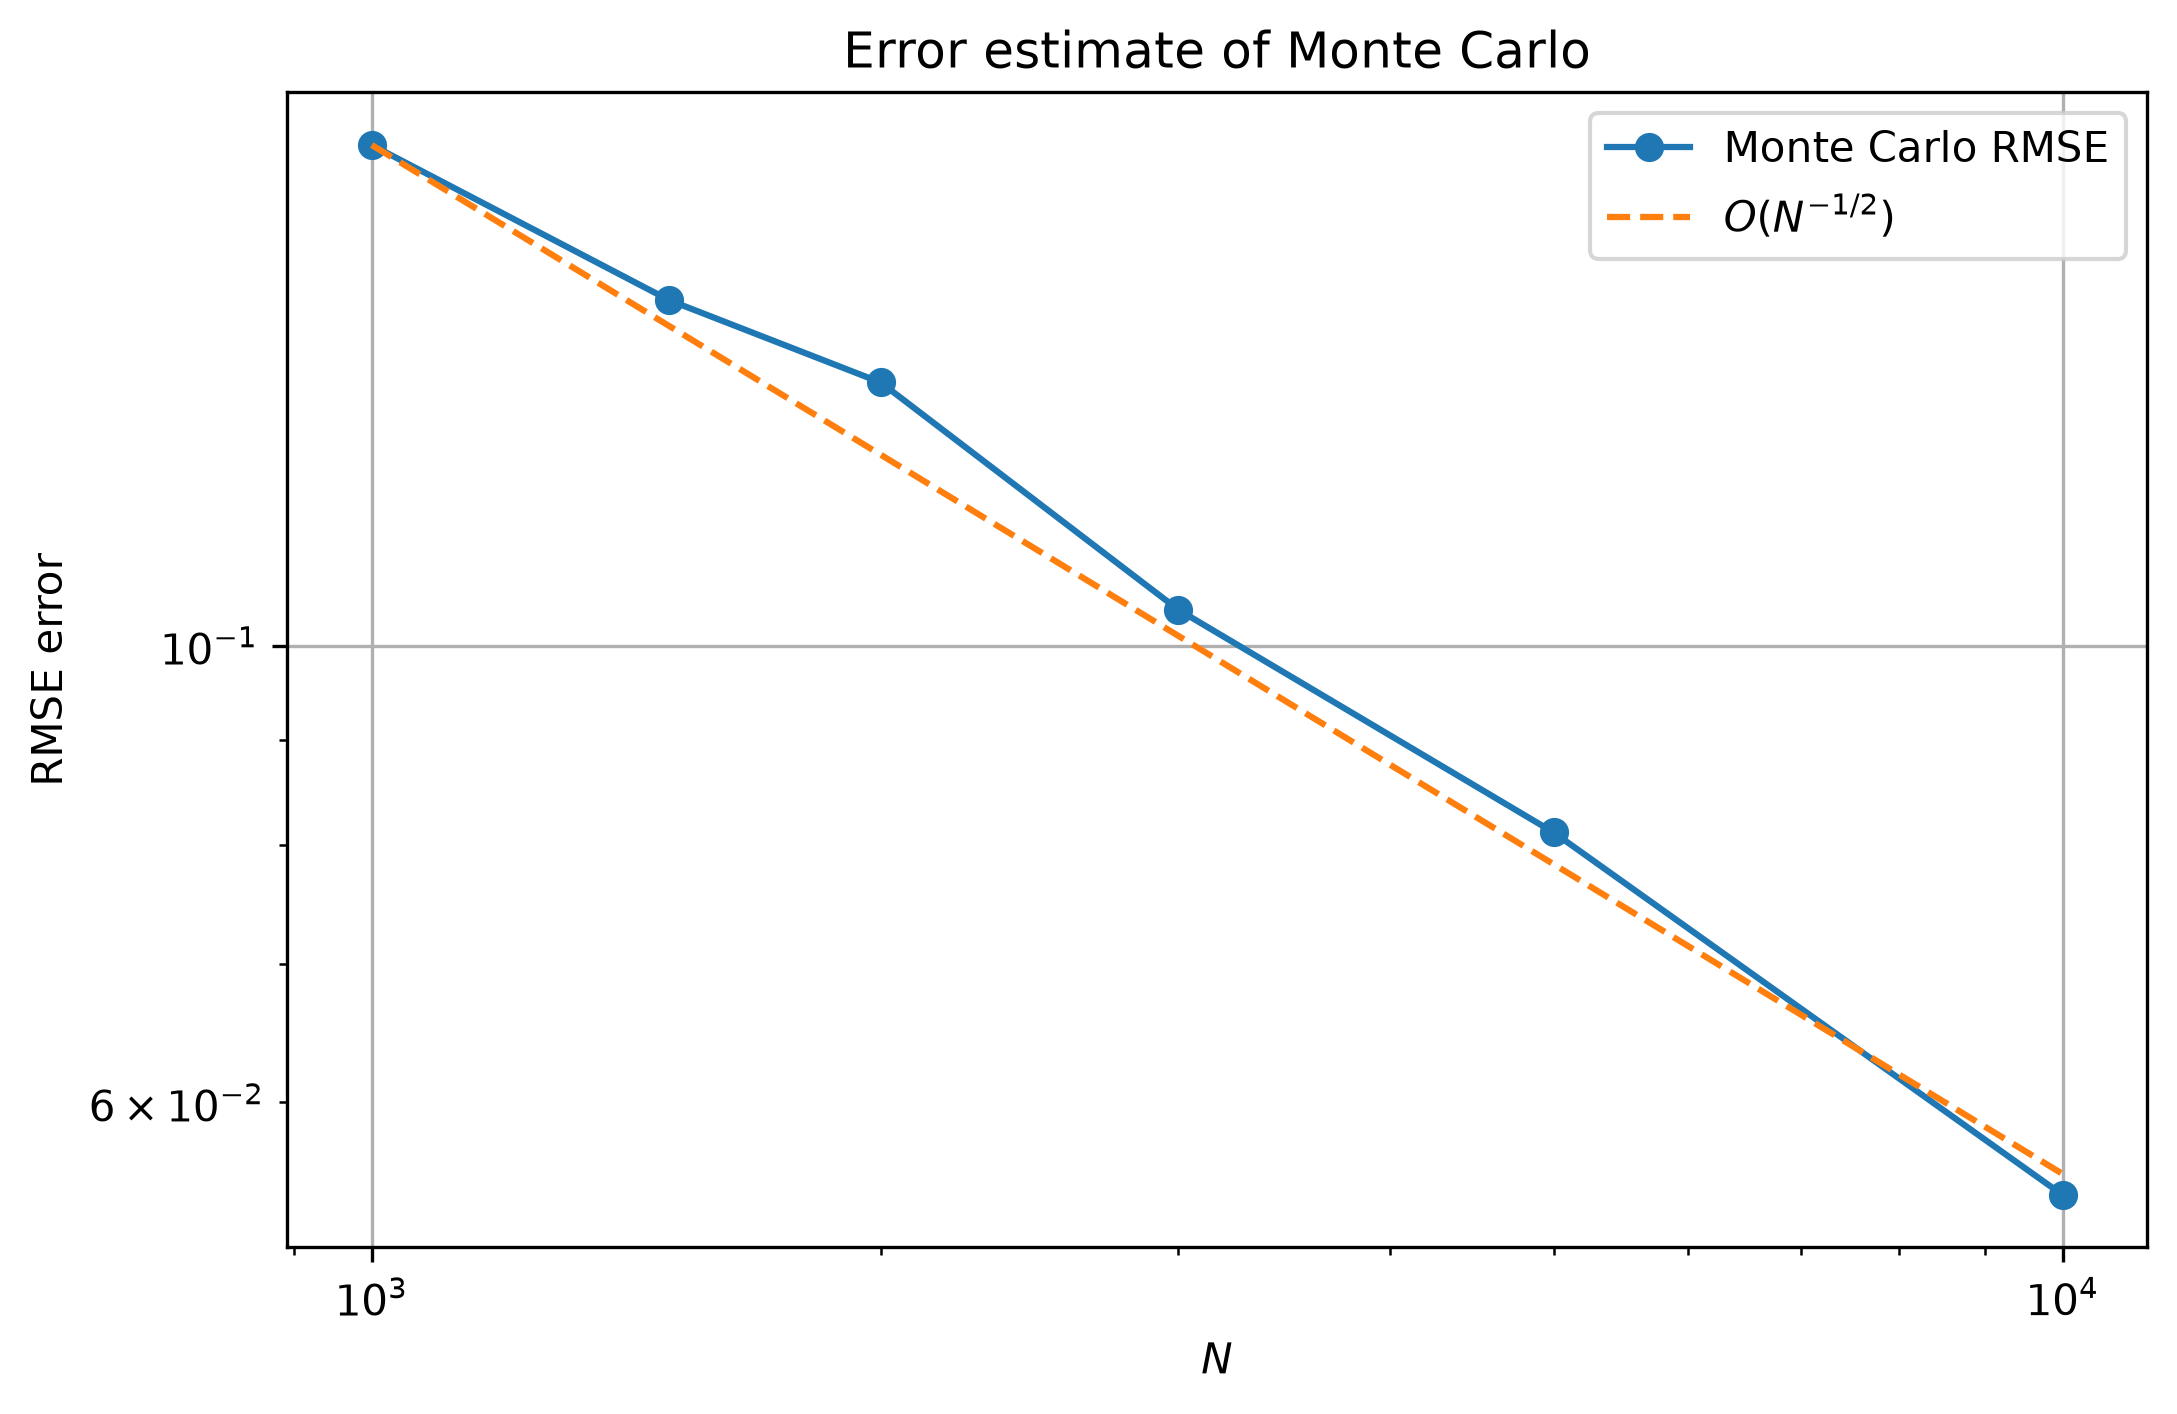
\includegraphics[width=0.82\textwidth]{01_mc_convergence.png}
\caption{Monte Carlo RMSE against the number of simulated paths. The fitted slope is approximately $-0.5144$.}
\label{fig:mc}
\end{figure}

The empirical rate is consistent with the standard Monte Carlo error scaling. In practical terms, reducing the RMSE by roughly one half requires about four times as many paths.

\subsection{Finite-difference PDE valuation}

The temporal experiment gives the following estimated orders:
\begin{table}[H]
\centering
\caption{Estimated temporal convergence orders from PDE self-convergence.}
\begin{tabular}{lrrrr}
\toprule
Scheme & Estimate 1 & Estimate 2 & Estimate 3 & Estimate 4\\
\midrule
Explicit & 1.0001 & 1.0000 & 1.0000 & 1.0000\\
Implicit & 0.9999 & 1.0000 & 1.0000 & 1.0000\\
Crank--Nicolson & 2.0000 & 2.0000 & 2.0020 & 1.9949\\
\bottomrule
\end{tabular}
\end{table}

With $M=100$ fixed, all three methods approach a price near $4.08513$ as the time step is refined. This is about $0.0150$ below the continuous Black--Scholes price $4.10013$. The remaining difference is attributable to the fixed spatial grid and finite computational domain; it does not contradict temporal convergence. The self-convergence comparison isolates the temporal discretization error.

\begin{figure}[H]
\centering
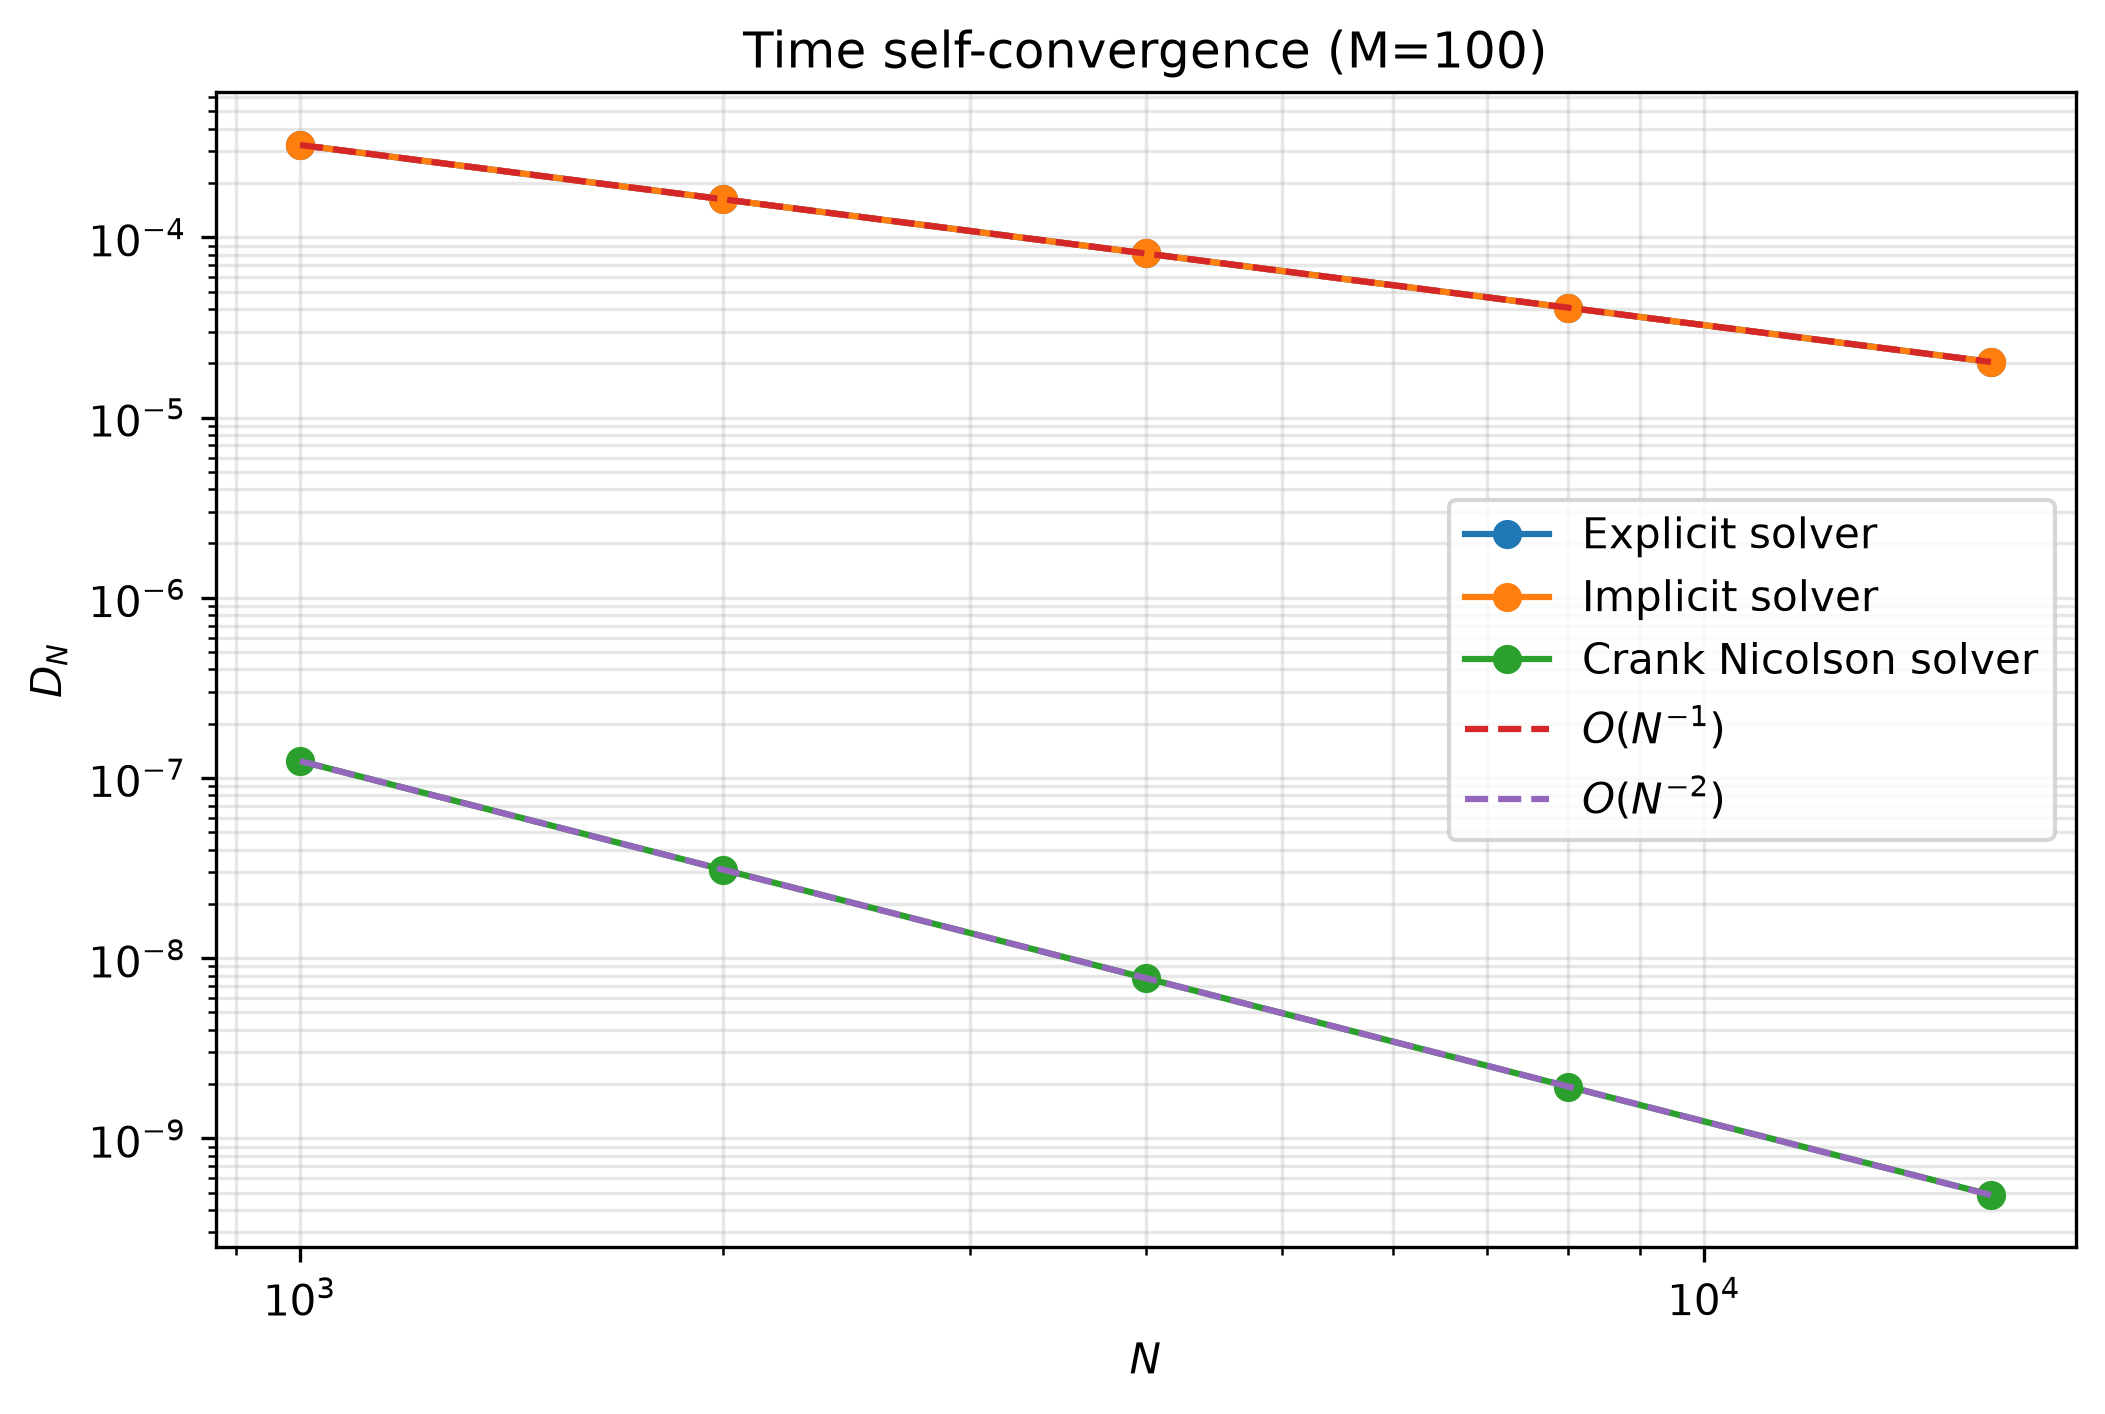
\includegraphics[width=0.88\textwidth]{02_pde_temporal_convergence.png}
\caption{Temporal convergence of the explicit, implicit, and Crank--Nicolson schemes.}
\label{fig:pde-time}
\end{figure}

For spatial convergence, the Crank--Nicolson price approaches the analytical benchmark as the spatial grid is refined. The observed orders are $2.0323$, $2.0074$, $2.0018$, and $2.0005$, supporting second-order spatial accuracy.

\begin{table}[H]
\centering
\caption{Crank--Nicolson spatial convergence.}
\begin{tabular}{rrrr}
\toprule
Spatial intervals $M$ & Numerical price & Absolute error & Estimated order\\
\midrule
40  & 4.00402727 & 0.09610443 & --\\
80  & 4.07663774 & 0.02349396 & 2.0323\\
160 & 4.09428843 & 0.00584327 & 2.0074\\
320 & 4.09867273 & 0.00145897 & 2.0018\\
640 & 4.09976707 & 0.00036463 & 2.0005\\
\bottomrule
\end{tabular}
\end{table}

\begin{figure}[H]
\centering
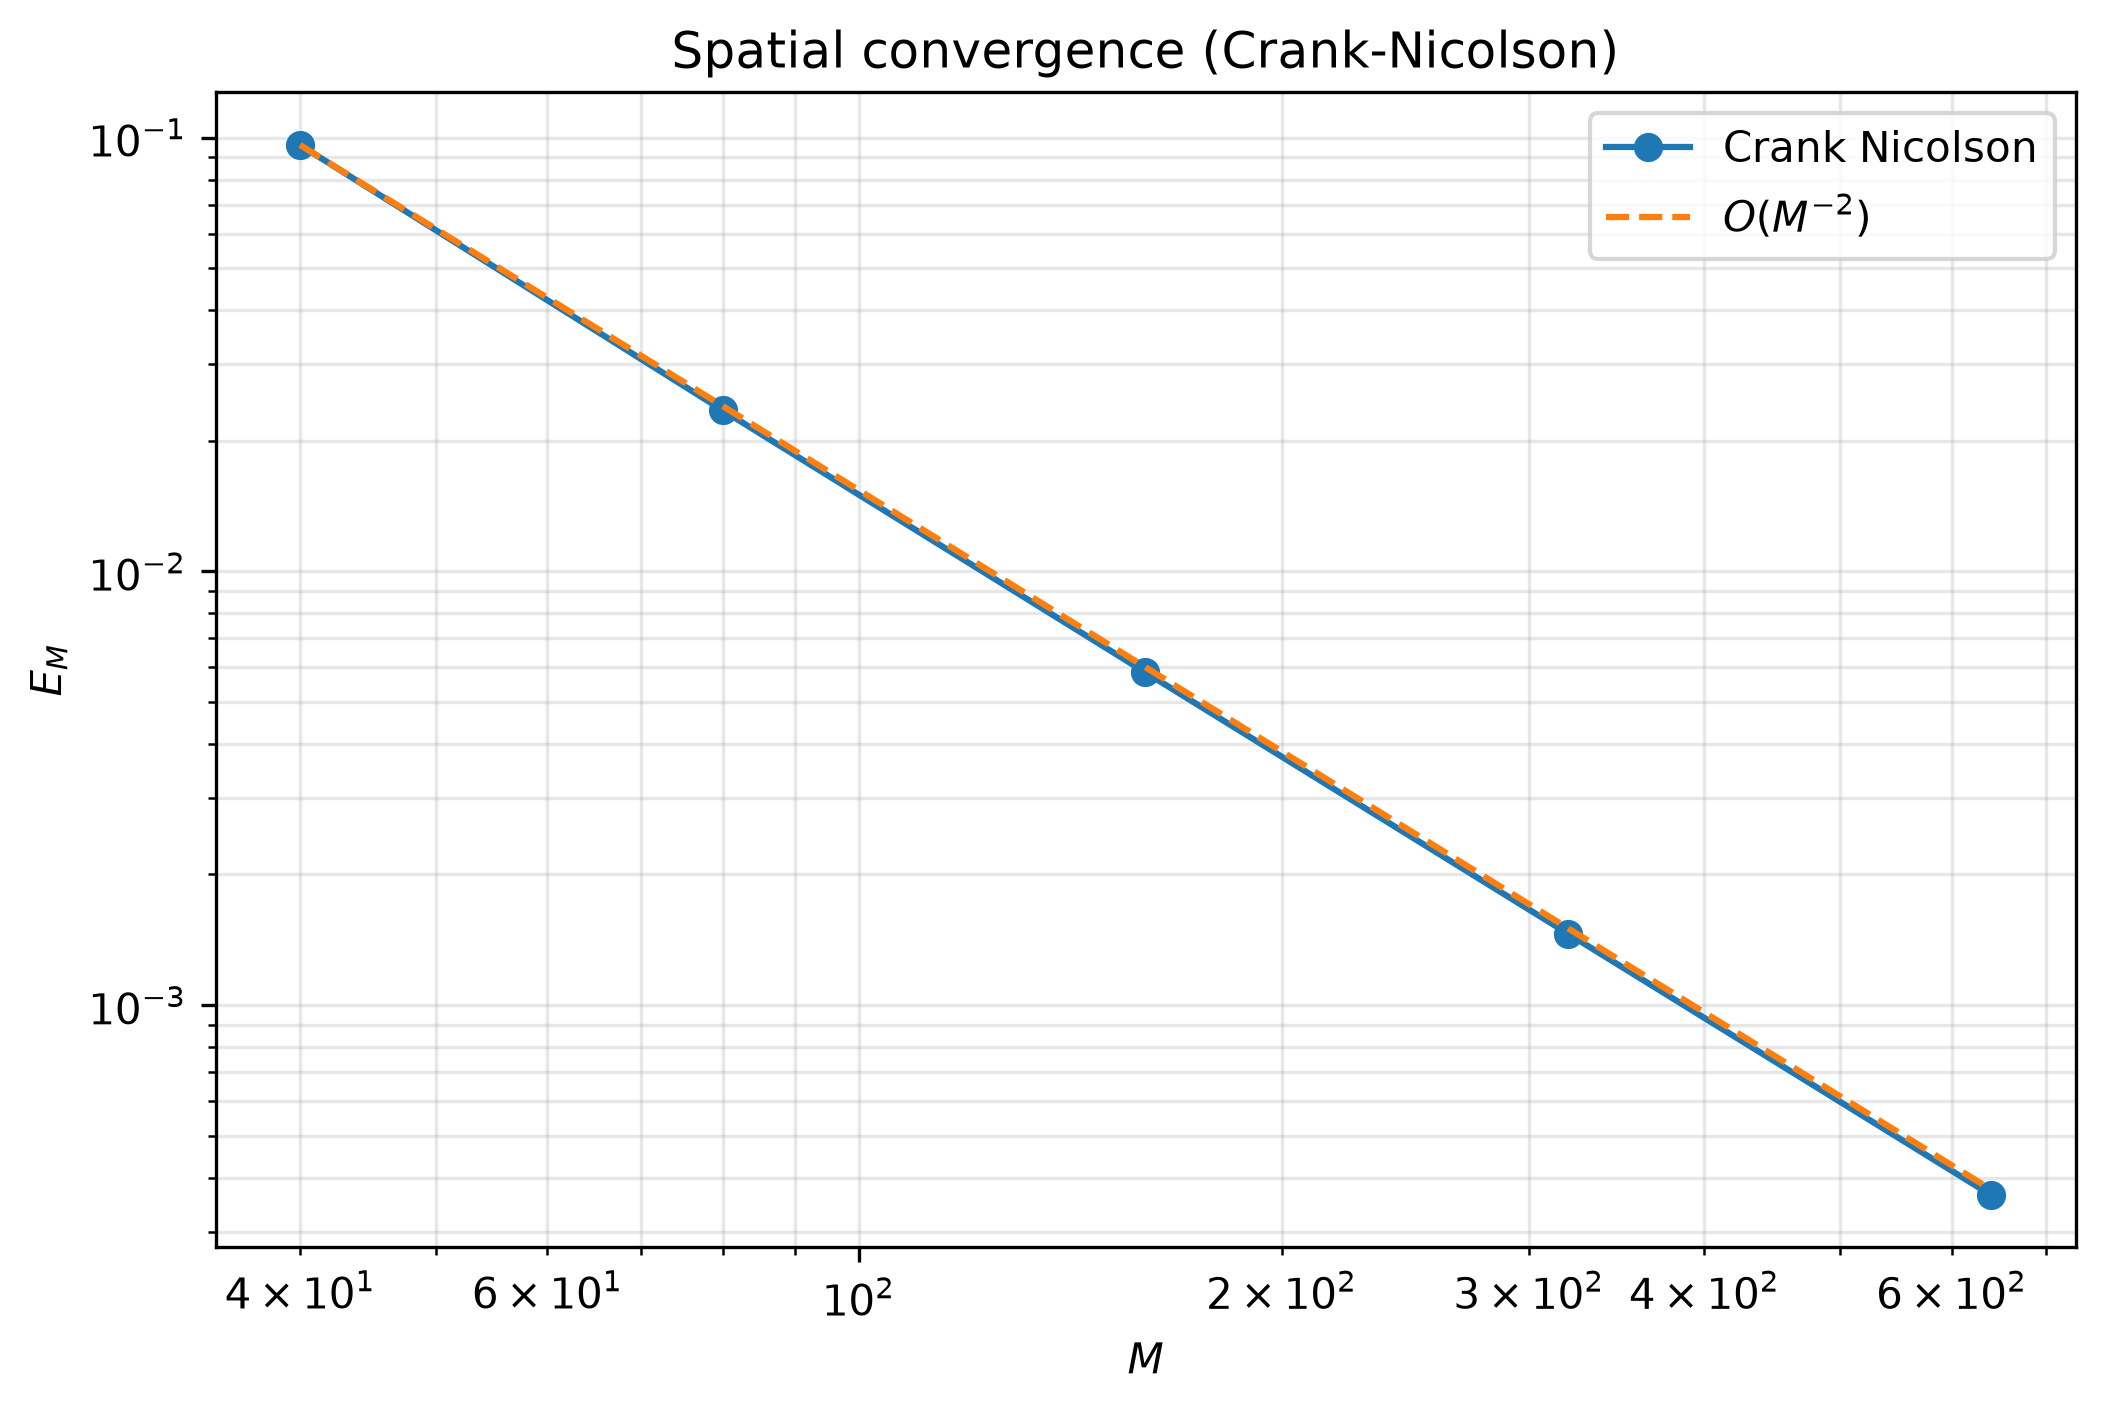
\includegraphics[width=0.88\textwidth]{02_pde_spatial_convergence.png}
\caption{Spatial convergence of the Crank--Nicolson scheme against the analytical Black--Scholes price.}
\label{fig:pde-space}
\end{figure}

The experiments confirm the expected first-order temporal accuracy of the explicit and implicit methods, second-order temporal accuracy of Crank--Nicolson, and second-order spatial accuracy of the central-difference discretization. Runtime comparisons are included in the notebook, but their absolute values are hardware- and implementation-dependent; they should not be interpreted as a controlled equal-accuracy benchmark.

\subsection{Delta and Vega}

For the base contract in (\ref{eq:baseparams}), the analytical values are
\[
\Delta_{\mathrm{BS}}=-0.38709562,\qquad
\Vega_{\mathrm{BS}}=12.34569149.
\]
Central bump-and-reprice estimates exhibit fitted convergence slopes of $1.9909$ for Delta and $2.0152$ for Vega, consistent with the second-order truncation error of central differences.

\begin{figure}[H]
\centering
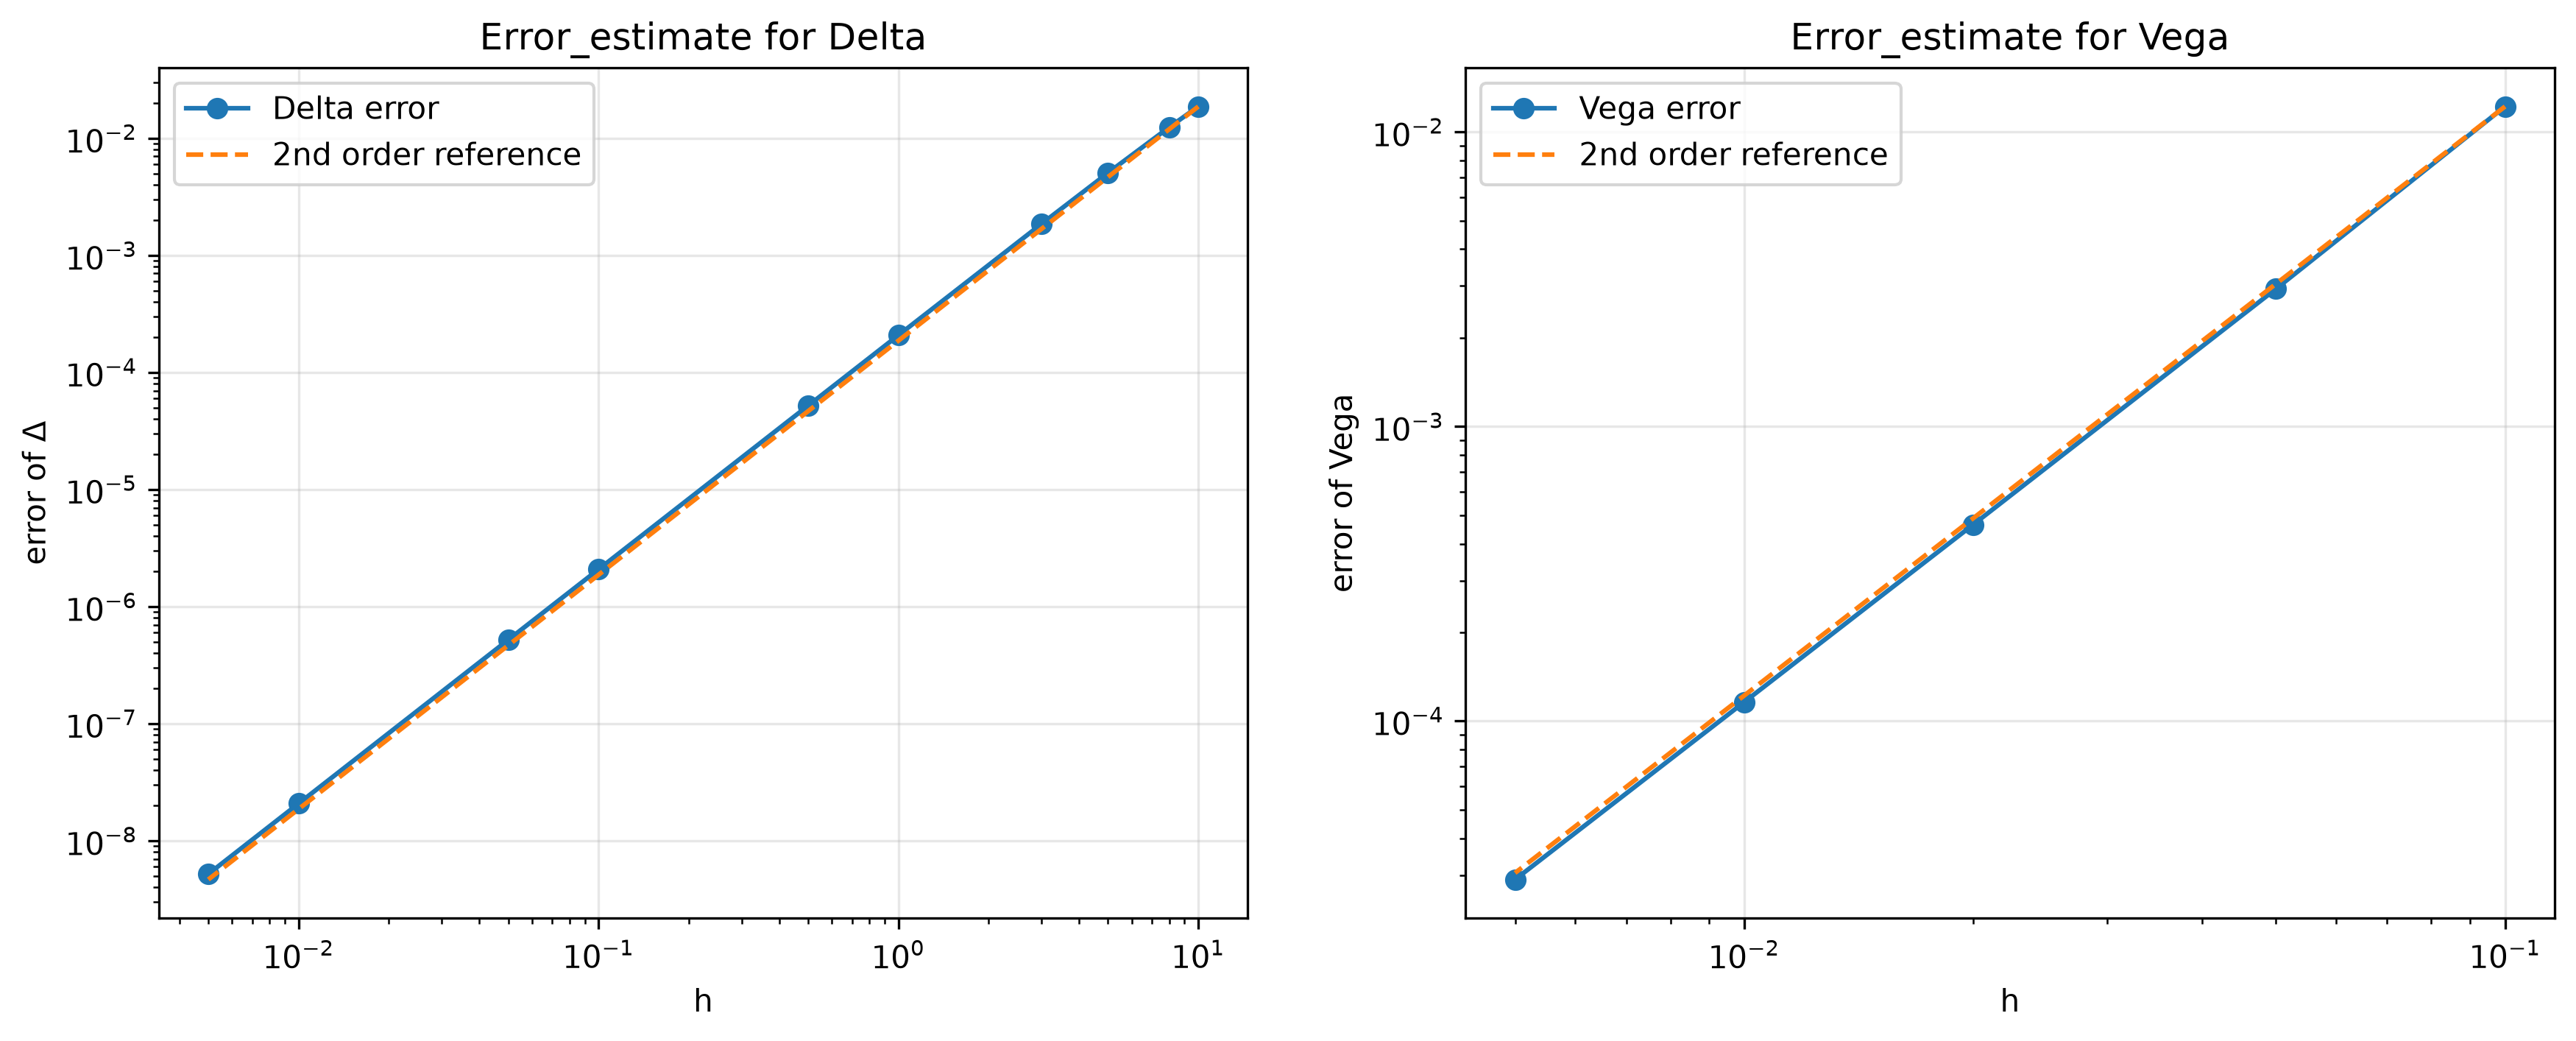
\includegraphics[width=\textwidth]{03_greeks_bump_convergence.png}
\caption{Central-difference bump-and-reprice convergence for Delta and Vega.}
\label{fig:greeks-bump}
\end{figure}

The Crank--Nicolson spatial experiment gives estimated orders of $1.9945$ for Delta and $2.0235$ for Vega. The volatility bump used for Vega is fixed at $\delta\sigma=0.001$. Consequently, the Vega estimate combines PDE discretization error with the error from numerical differentiation in volatility.

\begin{figure}[H]
\centering
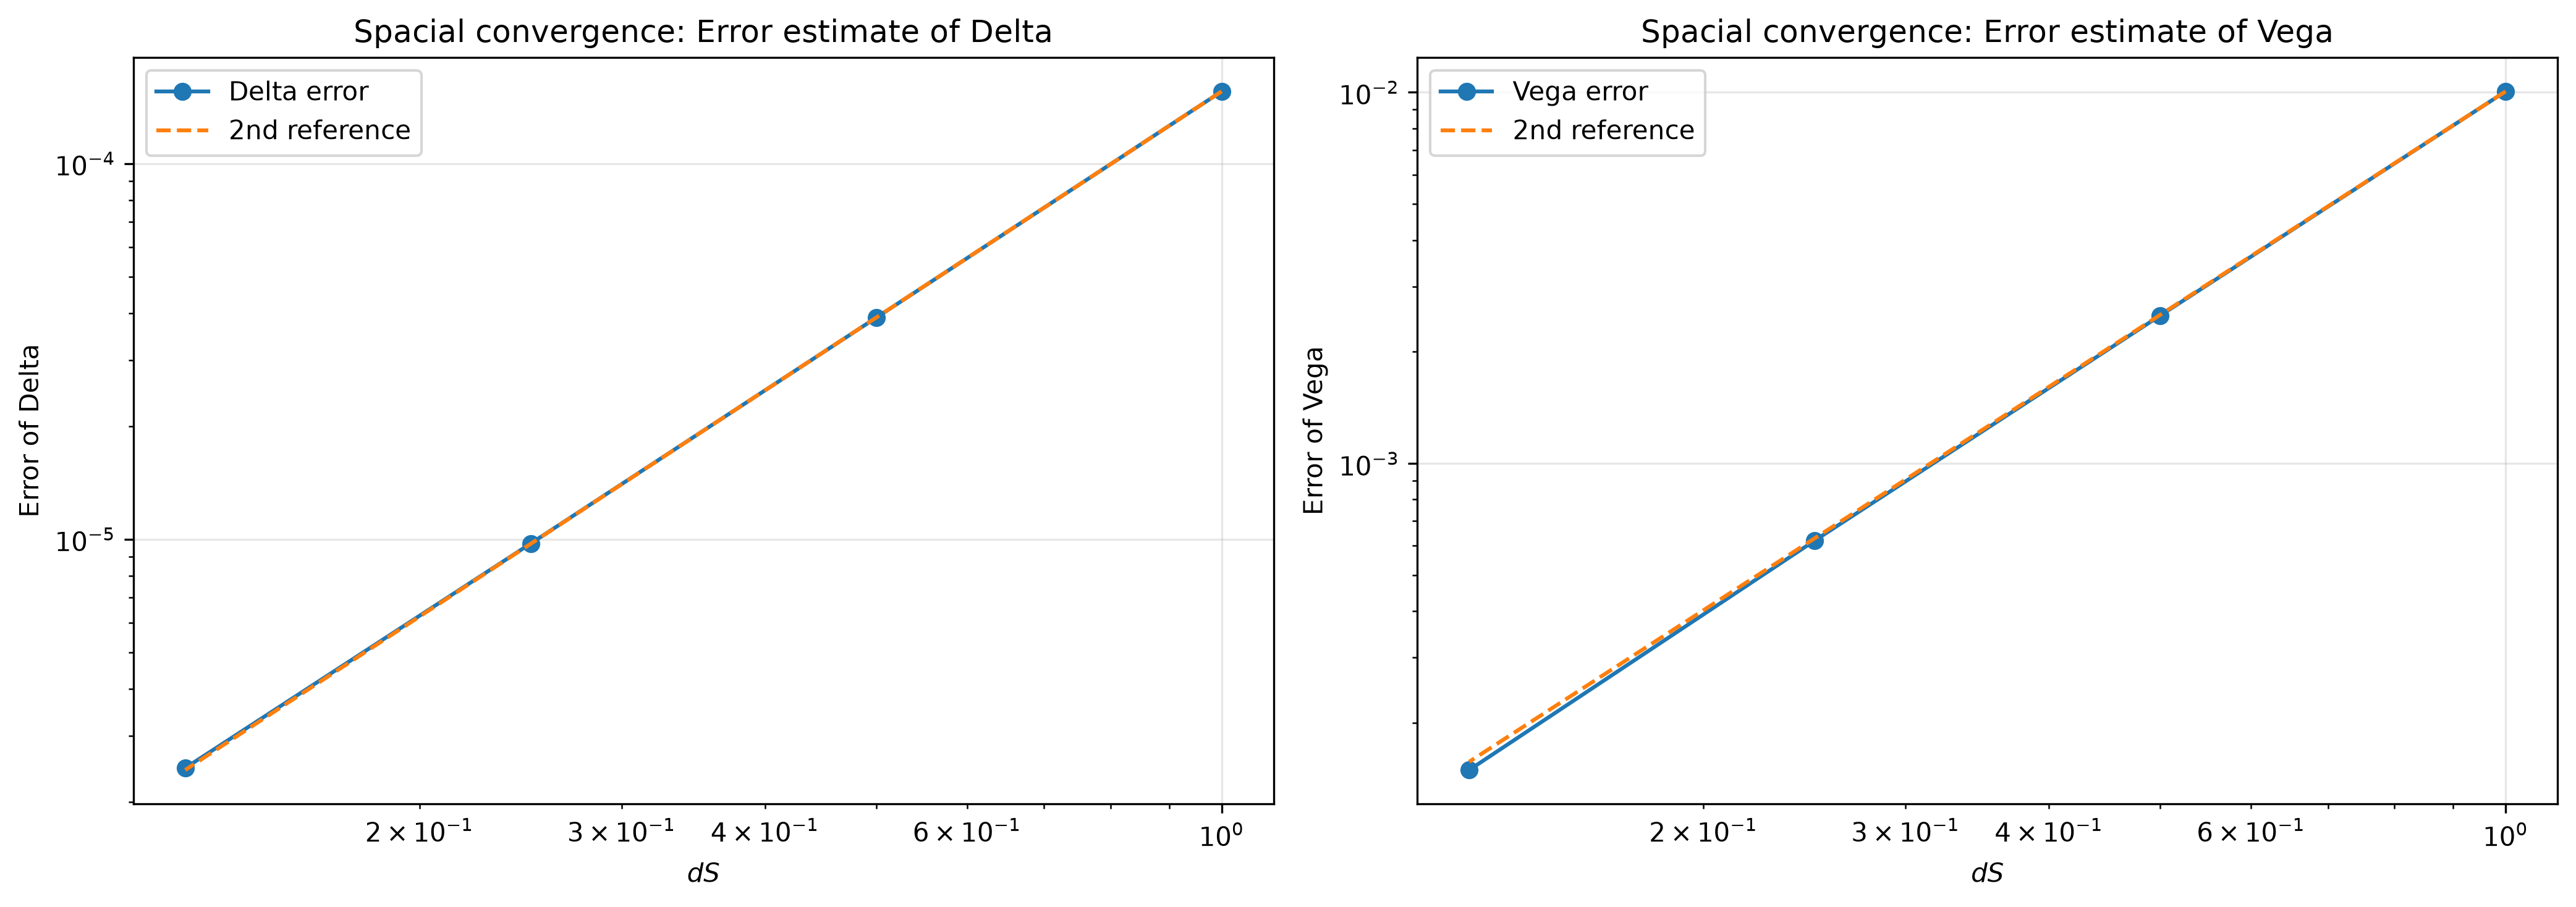
\includegraphics[width=\textwidth]{03_greeks_pde_convergence.png}
\caption{PDE-based Delta and Vega estimates under spatial and temporal grid refinement.}
\label{fig:greeks-pde}
\end{figure}

When the spatial grid is fixed at $M=800$ and the number of time steps increases, the Delta and Vega errors approach nonzero plateaus. This is expected: reducing the time step removes temporal discretization error but does not remove the remaining spatial error (or the fixed volatility-bump error in the Vega calculation).

\subsection{Implied-volatility inversion}

For the five synthetic prices generated from volatilities $0.2$, $0.4$, $0.6$, $0.8$, and $1.0$, both algorithms recover the prescribed values to the reported numerical tolerance. In the tested setup, Bisection takes 27 iterations for each case, while Newton takes 4 iterations from an initial guess of $0.3$.

\begin{table}[H]
\centering
\caption{Implied-volatility recovery from synthetic Black--Scholes prices.}
\begin{tabular}{rrrr}
\toprule
True volatility & Bisection estimate & Newton estimate & Iterations (Bisection / Newton)\\
\midrule
0.20 & 0.20000000 & 0.20000000 & 27 / 4\\
0.40 & 0.40000000 & 0.40000000 & 27 / 4\\
0.60 & 0.60000000 & 0.60000000 & 27 / 4\\
0.80 & 0.80000001 & 0.80000000 & 27 / 4\\
1.00 & 0.99999999 & 1.00000000 & 27 / 4\\
\bottomrule
\end{tabular}
\end{table}

Bisection provides a robust bracketing guarantee. If the initial volatility interval is $[a_0,b_0]$, the midpoint error satisfies
\[
|\sigma_n-\sigma_{\mathrm{imp}}|
\leq \frac{b_0-a_0}{2^n}.
\]
Newton is substantially faster in this example and displays local quadratic convergence, but its success depends on the initial guess and the magnitude of Vega.

\begin{figure}[H]
\centering
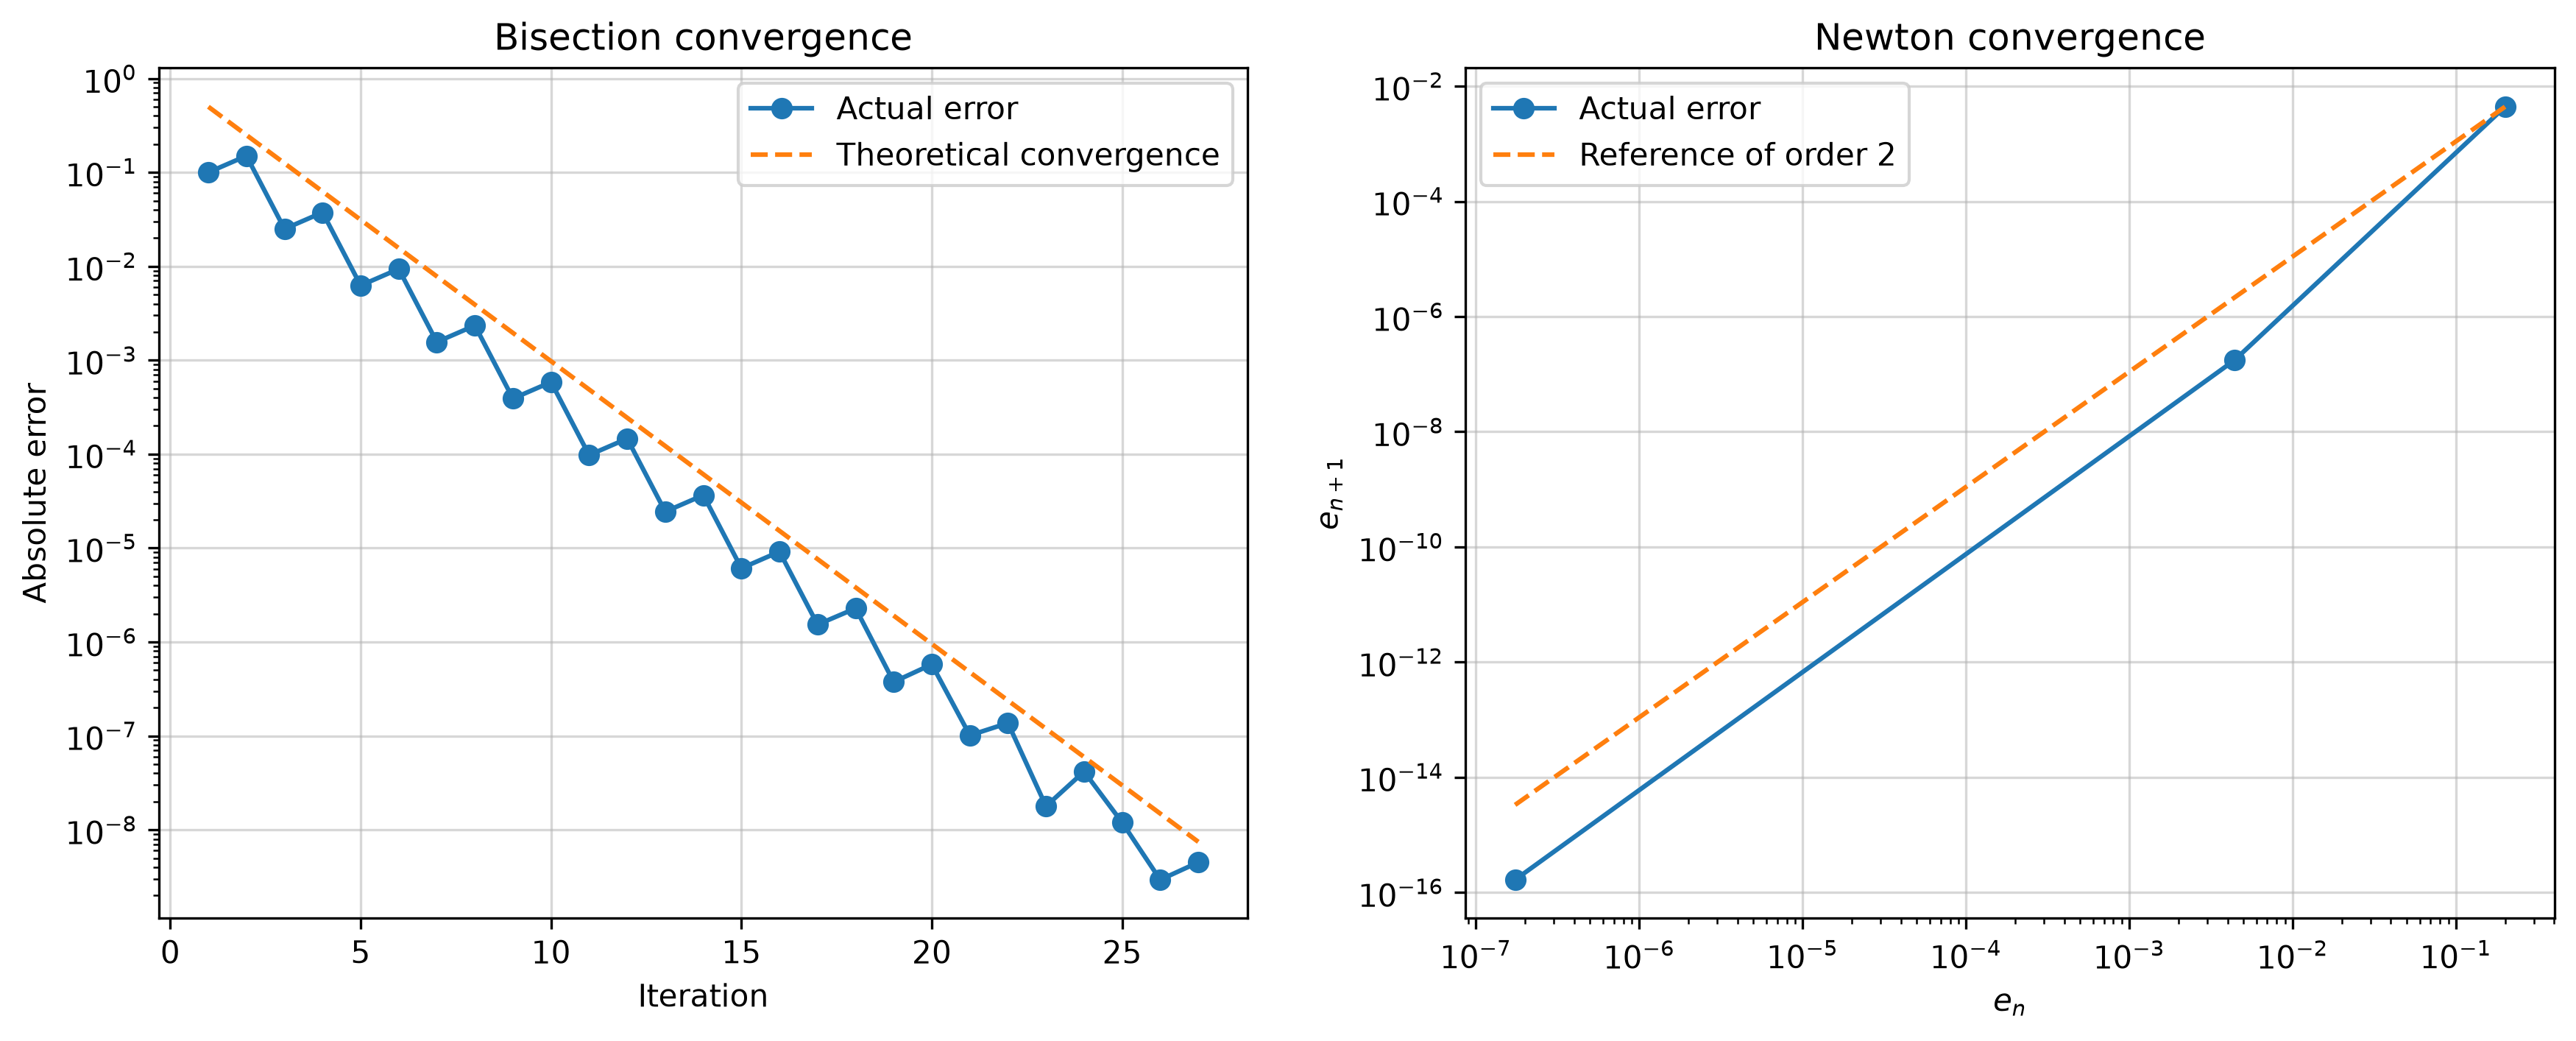
\includegraphics[width=\textwidth]{04_iv_solver_convergence.png}
\caption{Bisection and Newton convergence in the controlled implied-volatility experiment.}
\label{fig:iv-convergence}
\end{figure}

The stability experiment uses 100 combinations of strike, maturity, and initial volatility. With the dividend yield explicitly reset to $q=0.003$, 63 of the 100 cases meet the volatility-error criterion $|\widehat{\sigma}-\sigma_{\mathrm{true}}|<10^{-4}$. The tracking routine reports a price-tolerance stop in 73 cases, but 10 of those estimates still fail the volatility-error criterion. A further 23 cases terminate because Vega is too small and 4 because the Newton step is invalid. The heatmap reports the fraction of accurate recoveries across the five initial guesses for each $(K,T)$ pair.

\begin{figure}[H]
\centering
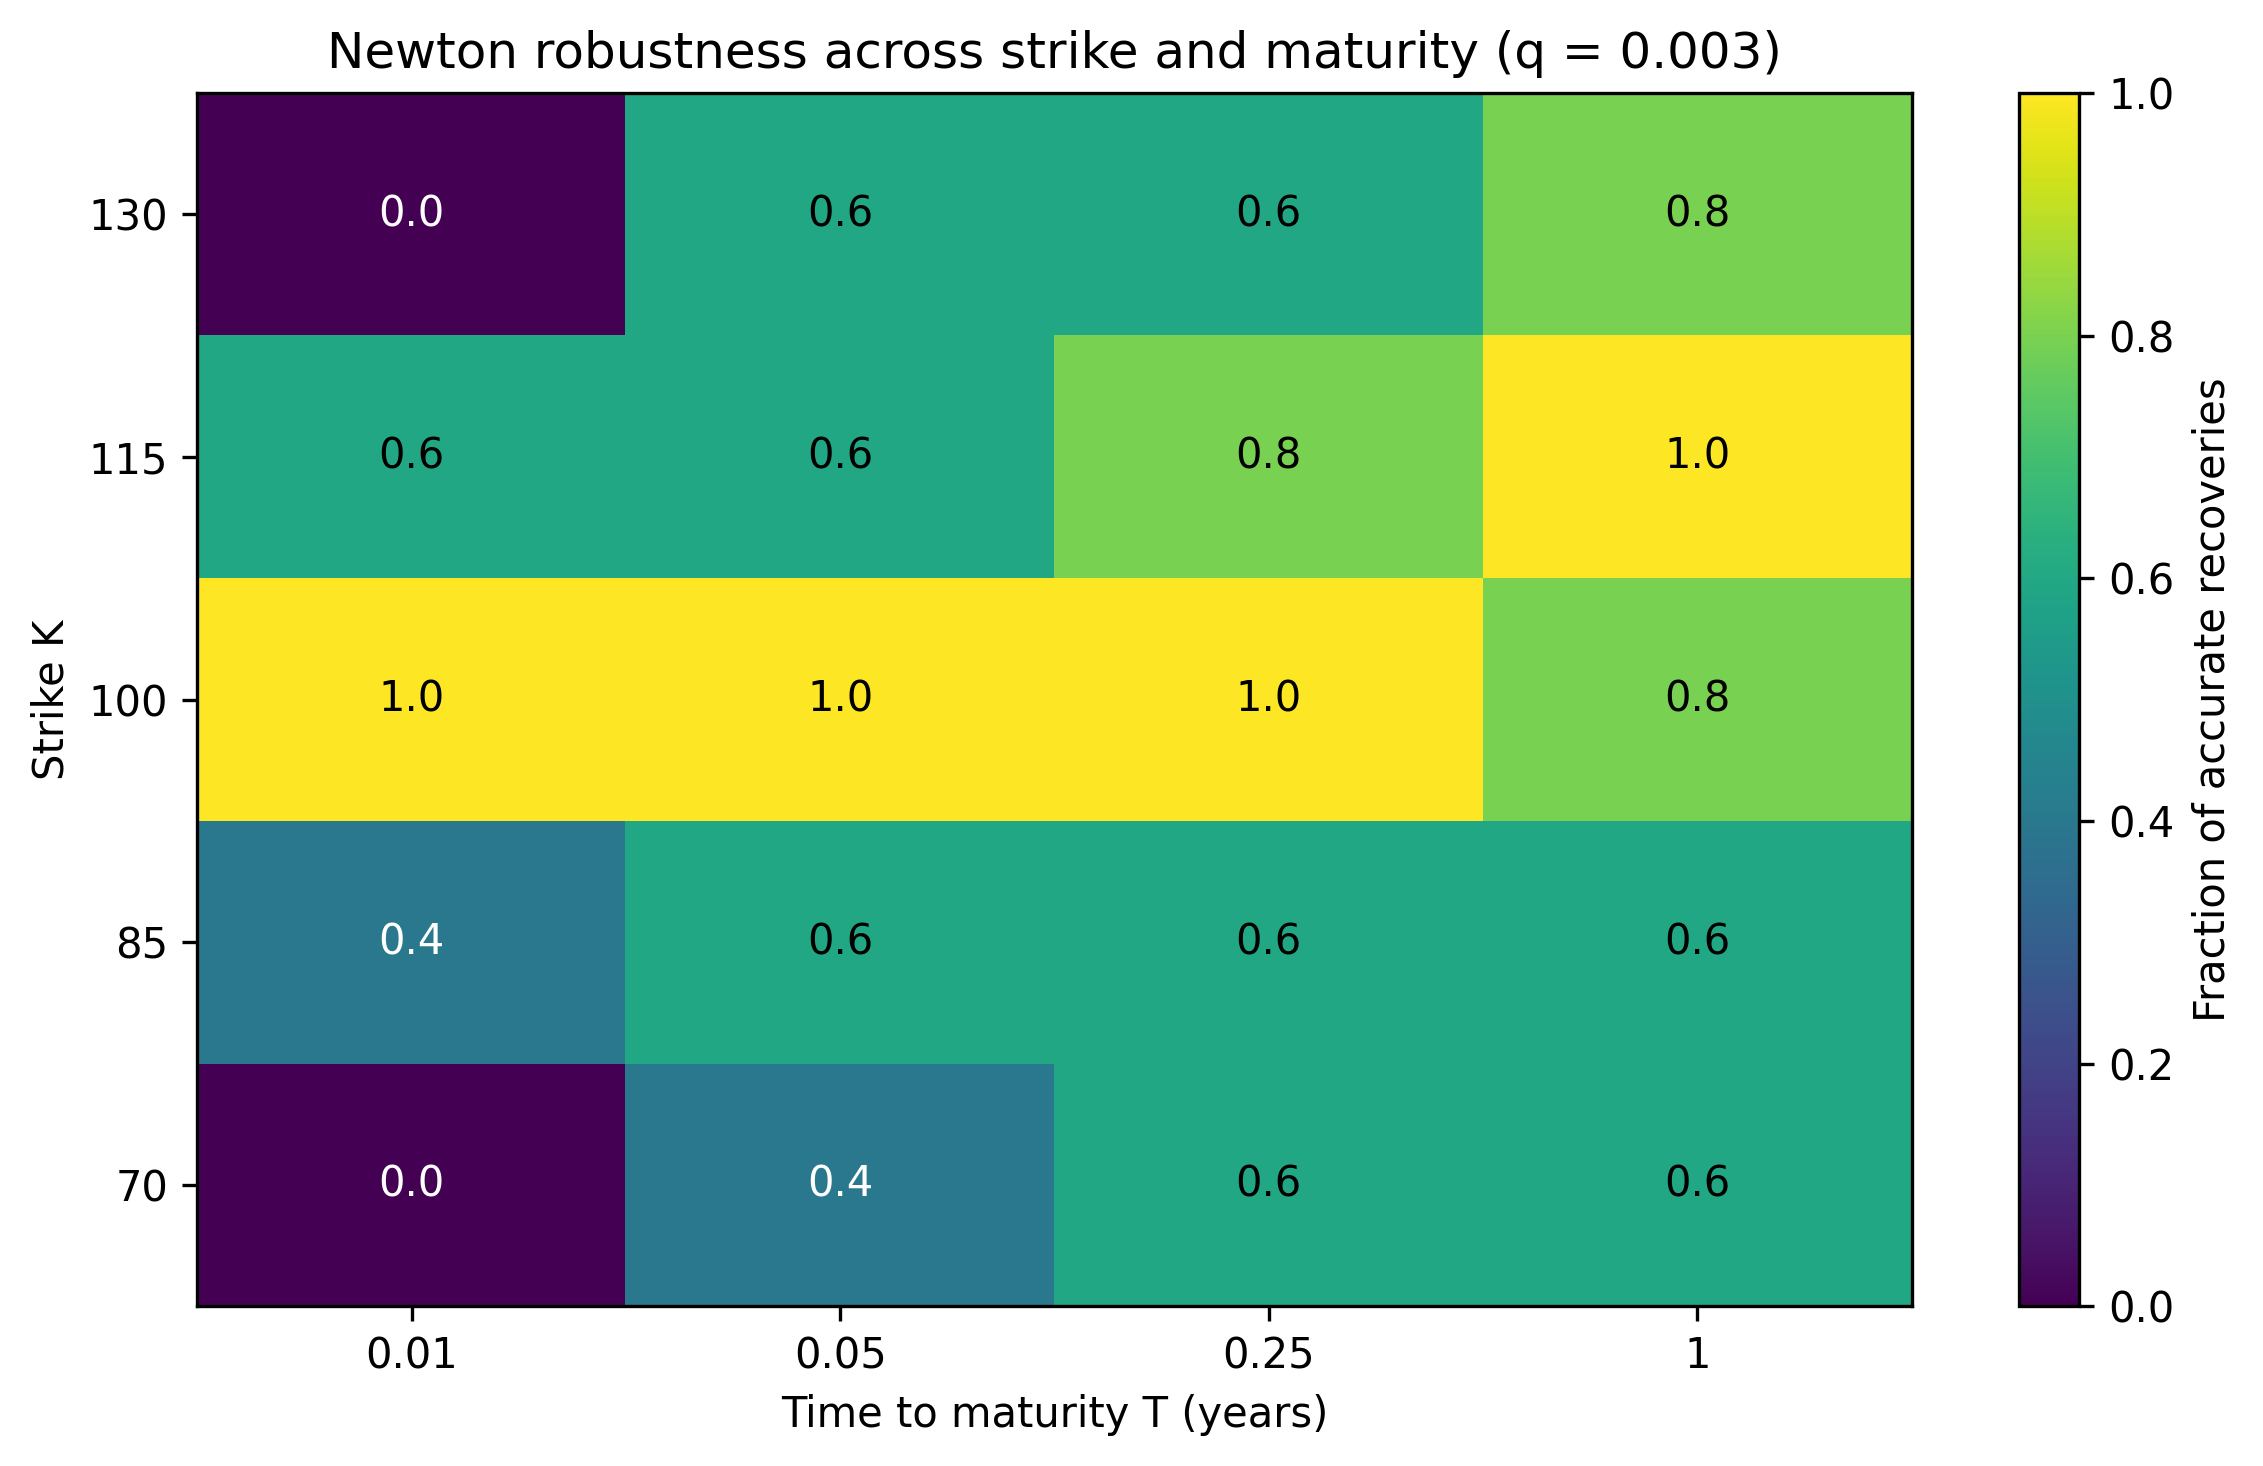
\includegraphics[width=0.82\textwidth]{04_newton_stability_heatmap.png}
\caption{Newton stability across strike and maturity. Each cell is the successful-recovery fraction across five initial volatility guesses; the experiment uses $q=0.003$.}
\label{fig:iv-stability}
\end{figure}

A small pricing residual does not necessarily imply an accurate implied-volatility estimate. By implicit differentiation,
\begin{equation}
  \frac{\partial \sigma_{\mathrm{imp}}}{\partial P_{\mathrm{mkt}}}
  =\frac{1}{\Vega}.
\end{equation}
When Vega is close to zero, even a small price error can correspond to a material volatility error. This explains why price-based stopping criteria should be interpreted together with the recovered-volatility error and the local Vega.

\section{AAPL Implied-Volatility Analysis}

\subsection{Data and market inputs}

The final experiment uses a Yahoo Finance AAPL option-chain snapshot dated 6 November 2026. The underlying reference price is set to $S_0=\$342.36$, consistent with the 15:59 one-minute close on that date. The continuous dividend yield is set to $q=0.00315$, based on an annual dividend assumption of \$1.08. Maturity-dependent risk-free rates are derived from the saved U.S. Treasury yield data using the project's interpolation procedure.

The option-chain file contains 2,152 contracts across 16 expiration dates, spanning 21 to 805 calendar days. After basic cleaning, 1,945 contracts remain, of which 984 are classified as out-of-the-money (OTM). The implied-volatility inversion uses option mid-quotes and Brent's bracketing root finder. With a 30\% relative bid--ask spread limit, 1,545 cleaned contracts enter the IV calculation and 1,523 receive a numerical solution, a 98.58\% success rate. For the OTM subset, all 584 contracts within the 30\% limit receive an IV solution.

\subsection{Spread filtering and volatility smile}

The main smile, term-structure, and surface plots use a 20\% relative bid--ask spread threshold. This retains 500 OTM observations. For comparison, the OTM sample sizes under 10\%, 15\%, 20\%, and 30\% spread limits are 344, 434, 500, and 584, respectively. The 20\% cutoff is a practical compromise between quote filtering and cross-maturity coverage, not a universally optimal threshold.

\begin{figure}[H]
\centering
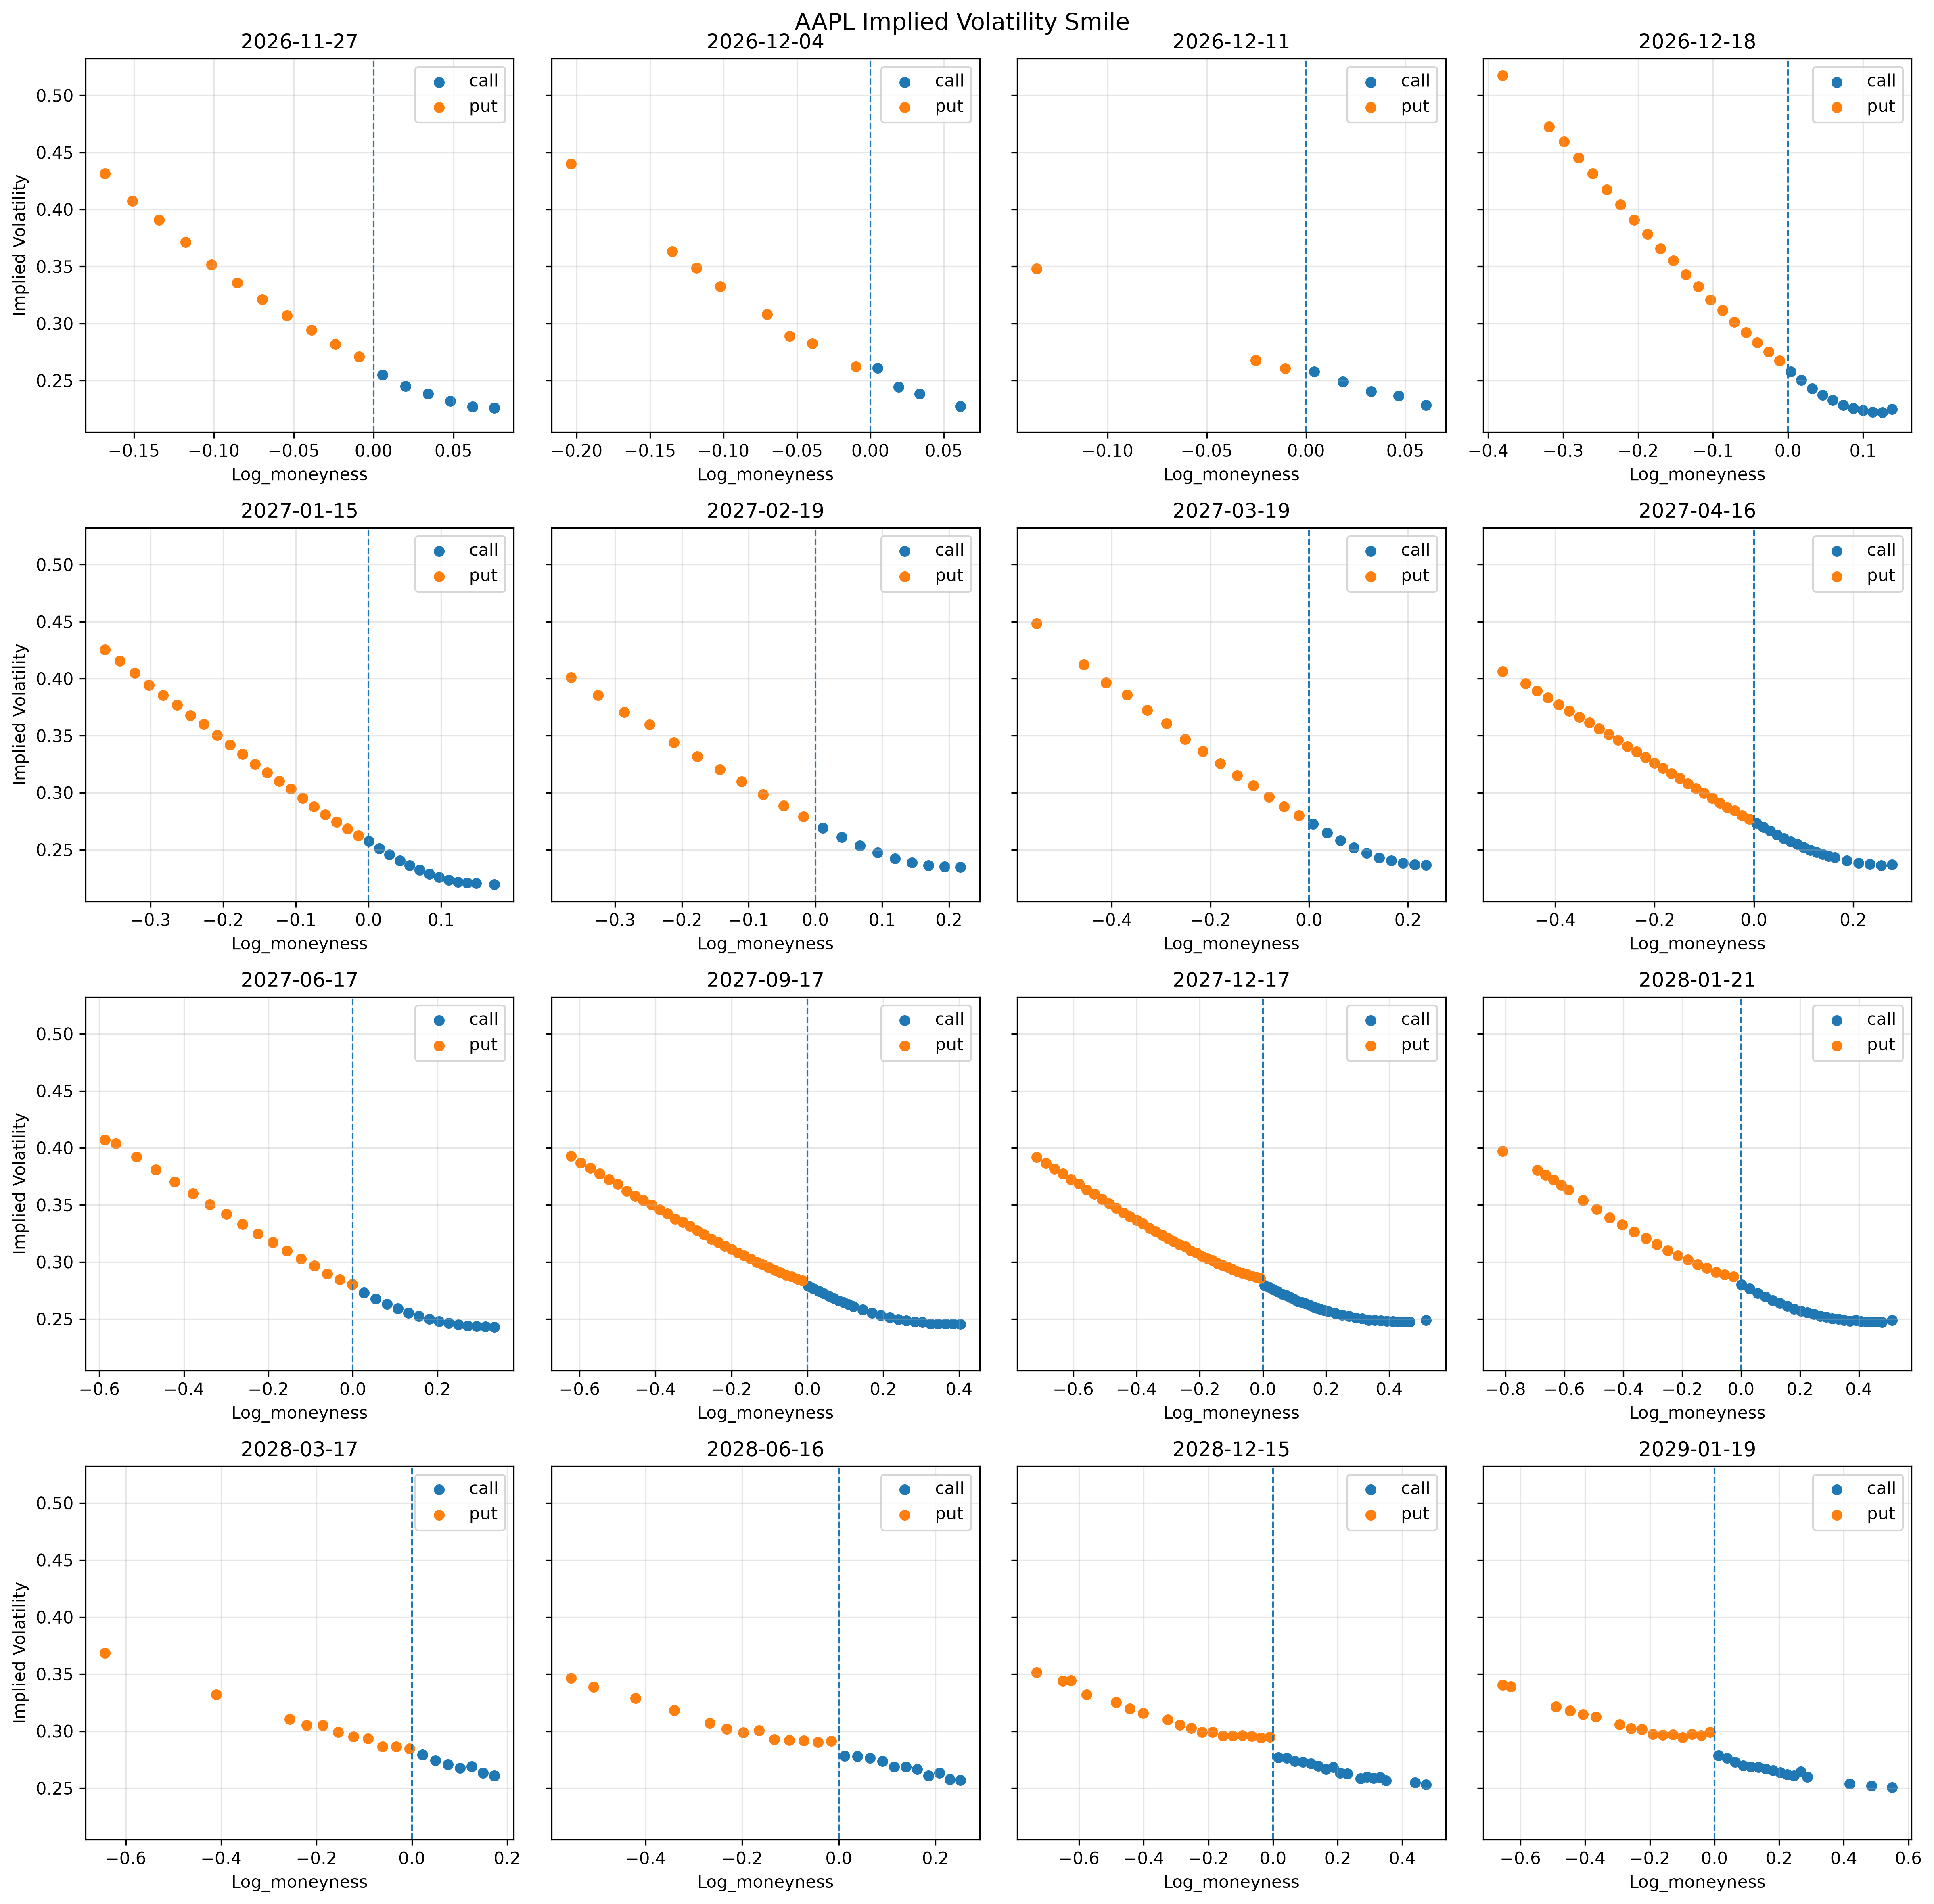
\includegraphics[width=0.90\textwidth,height=0.56\textheight,keepaspectratio]{05_AAPL_volatility_smile.png}
\caption{AAPL implied-volatility smiles across the selected expirations, using OTM contracts and a 20\% relative-spread filter.}
\label{fig:aapl-smile}
\end{figure}

The smiles show a negative equity skew for most expirations: lower-strike OTM puts generally carry higher implied volatility than higher-strike OTM calls. The plots should be read as a cross-section of filtered quotes rather than as a fitted parametric smile model.

\subsection{ATM-forward term structure and surface}

For each expiration, the ATM-forward implied volatility is estimated by linear interpolation between the two observations that bracket zero log-moneyness. All 16 selected expirations have observations on both sides of the target in the filtered sample. The estimated term structure starts at approximately 26.10\% for the 21-day maturity, reaches a local low of approximately 25.77\% at 70 days, and then generally rises to approximately 28.83\% at 805 days. The term structure is not monotonic and contains local fluctuations.

\begin{figure}[H]
\centering
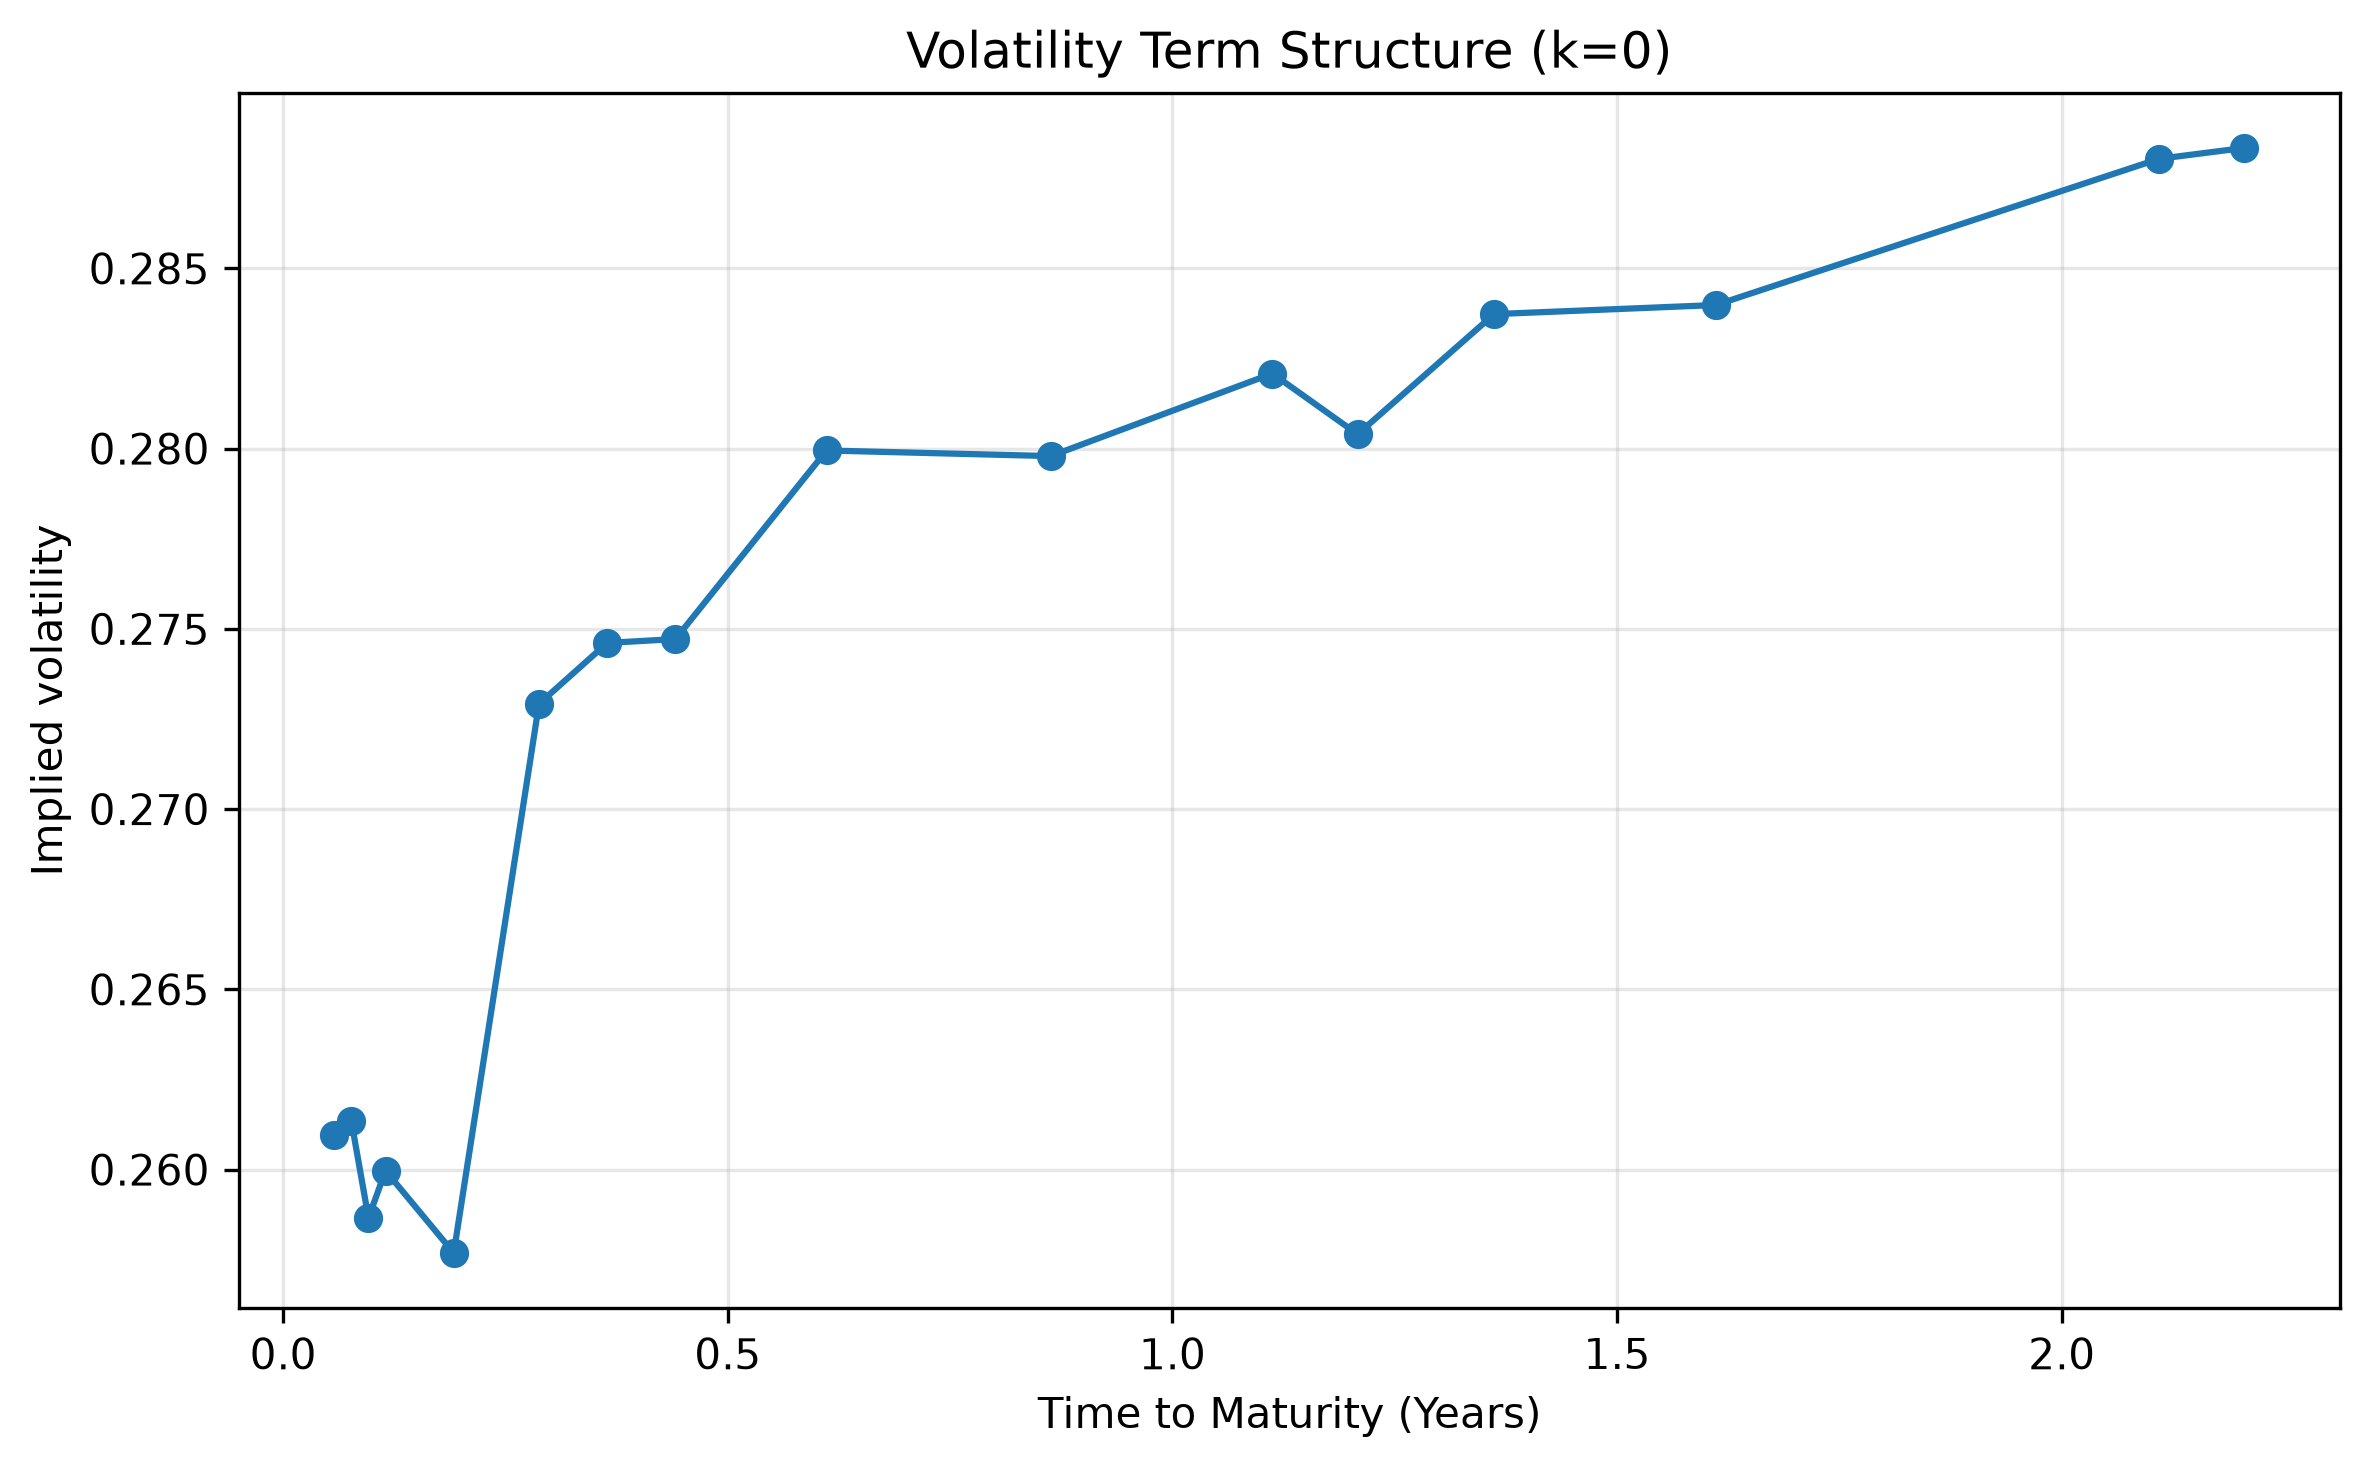
\includegraphics[width=0.88\textwidth]{05_AAPL_term_structure.png}
\caption{AAPL ATM-forward implied-volatility term structure, obtained by interpolation at zero log-moneyness.}
\label{fig:aapl-term}
\end{figure}

The spread-sensitivity comparison shows that the 15\%, 20\%, and 30\% filters produce the same ATM-forward estimates for most maturities. A visible difference occurs at the 11 December 2026 expiration: the 15\% filter gives approximately 25.65\%, compared with approximately 25.87\% under the 20\% and 30\% filters. The difference is modest, but it illustrates how a small number of available quotes can affect short-maturity estimates.

\begin{figure}[H]
\centering
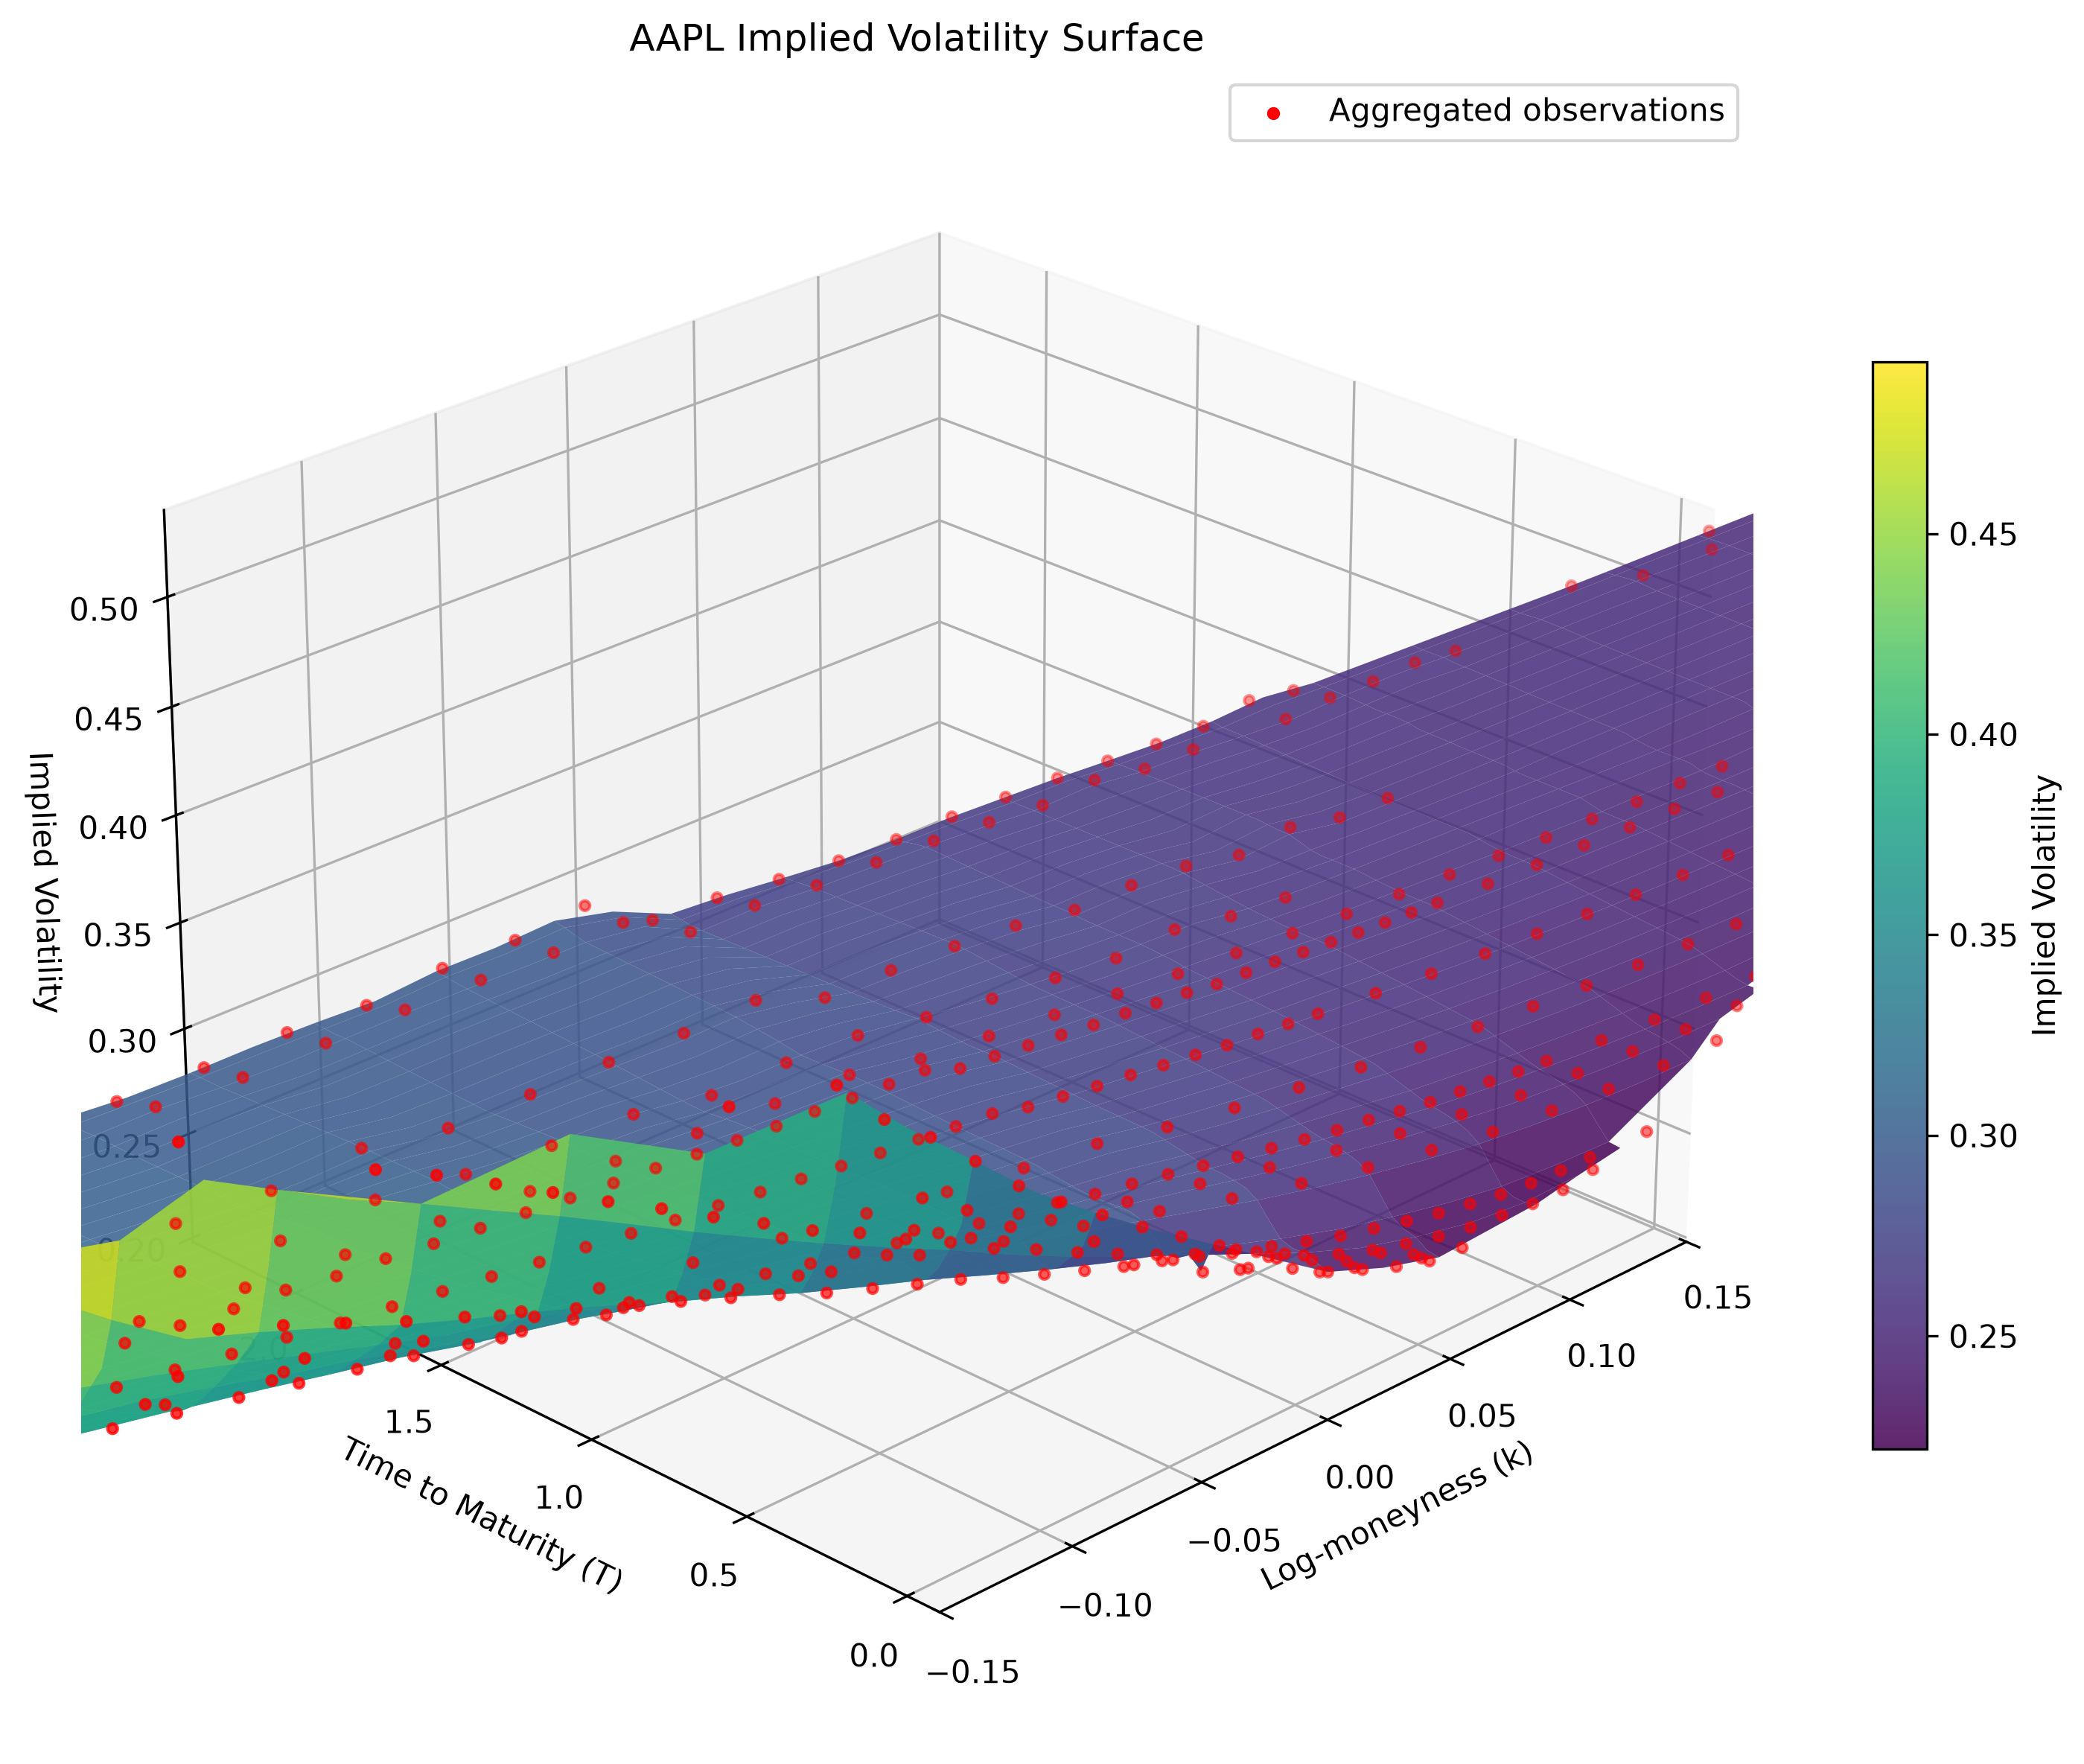
\includegraphics[width=0.82\textwidth,height=0.54\textheight,keepaspectratio]{05_AAPL_volatility_surface.png}
\caption{Interpolated AAPL implied-volatility surface over log-moneyness and time to maturity.}
\label{fig:aapl-surface}
\end{figure}

The three-dimensional surface is produced by piecewise-linear interpolation of the observed implied-volatility points. It is a visualization of the sampled data and is not an arbitrage-free surface calibration or a forecasting model.

\subsection{Limitations of the market-data analysis}

Several limitations should be kept in mind:
\begin{itemize}
  \item AAPL listed equity options are American-style, whereas the inversion uses the European Black--Scholes formula as an approximation.
  \item A constant continuous dividend yield approximates discrete cash dividends.
  \item The risk-free inputs are based on Treasury par yields and the project's interpolation procedure, rather than a bootstrapped zero-coupon curve. For maturities shorter than the shortest available Treasury tenor, the routine uses the first available tenor's rate.
  \item The stock reference price is close to the 15:59 close, but a reliable timestamp for every individual option bid and ask is unavailable. Exact synchronization between the stock and option quotes cannot be guaranteed.
  \item Relative-spread filtering is a practical quote-quality screen. It does not eliminate stale quotes, low liquidity, or all microstructure effects.
  \item The interpolated surface is not constrained to satisfy static-arbitrage conditions.
\end{itemize}

\section{Conclusion}

The five experiments form a progression from model-based option valuation to a market-data application. The Monte Carlo experiment reproduces the expected $N^{-1/2}$ RMSE scaling. The finite-difference experiments verify first-order temporal convergence for explicit and implicit schemes, second-order temporal convergence for Crank--Nicolson, and second-order spatial convergence. The Greeks experiments show that central differences can accurately recover Delta and Vega when the grid and bump sizes are appropriately chosen. The implied-volatility experiments illustrate the speed of Newton's method and the robustness advantage of Bisection, while also showing that low Vega can make volatility inversion ill-conditioned.

The AAPL application demonstrates a practical sequence of quote cleaning, spread filtering, implied-volatility calculation, and visualization. It also highlights that market-implied volatility estimates depend on quote quality, contract exercise style, dividend and rate assumptions, and the method used to interpolate the surface.

Overall, the project provides a hands-on foundation in option pricing, numerical PDE methods, risk sensitivities, root finding, and empirical implied-volatility analysis. The implementation is intended for learning and experimentation, not for production valuation, arbitrage-free calibration, or investment recommendations.

\section*{Reproducibility Notes}
\addcontentsline{toc}{section}{Reproducibility Notes}
The numerical results in this report are based on the supplied notebooks and saved figures. Two mathematical details should be kept consistent when reproducing the experiments:
\begin{enumerate}
  \item In the PDE notebook, the implicit and Crank--Nicolson drift coefficients in the written derivation should use $(r-q)$, consistent with the implemented solver. The discount term continues to use $r$. The saved \texttt{pde\_solver.py} implementation already follows this convention.
  \item For Bisection, let $p_n$ denote the midpoint evaluated at the $n$th iteration. The interval before that iteration has length $(b_0-a_0)/2^{n-1}$, so the midpoint error satisfies
  \[
    |p_n-p^*|\leq \frac{b_0-a_0}{2^n}.
  \]
  The theoretical reference curve in the IV convergence figure uses this bound.
\end{enumerate}

\end{document}
